\documentclass[twoside]{book}

% Packages required by doxygen
\usepackage{calc}
\usepackage{doxygen}
\usepackage{graphicx}
\usepackage[utf8]{inputenc}
\usepackage{makeidx}
\usepackage{multicol}
\usepackage{multirow}
\usepackage{textcomp}
\usepackage[table]{xcolor}

% Font selection
\usepackage[T1]{fontenc}
\usepackage{mathptmx}
\usepackage[scaled=.90]{helvet}
\usepackage{courier}
\usepackage{amssymb}
\usepackage{sectsty}
\renewcommand{\familydefault}{\sfdefault}
\allsectionsfont{%
  \fontseries{bc}\selectfont%
  \color{darkgray}%
}
\renewcommand{\DoxyLabelFont}{%
  \fontseries{bc}\selectfont%
  \color{darkgray}%
}

% Page & text layout
\usepackage{geometry}
\geometry{%
  a4paper,%
  top=2.5cm,%
  bottom=2.5cm,%
  left=2.5cm,%
  right=2.5cm%
}
\tolerance=750
\hfuzz=15pt
\hbadness=750
\setlength{\emergencystretch}{15pt}
\setlength{\parindent}{0cm}
\setlength{\parskip}{0.2cm}
\makeatletter
\renewcommand{\paragraph}{%
  \@startsection{paragraph}{4}{0ex}{-1.0ex}{1.0ex}{%
    \normalfont\normalsize\bfseries\SS@parafont%
  }%
}
\renewcommand{\subparagraph}{%
  \@startsection{subparagraph}{5}{0ex}{-1.0ex}{1.0ex}{%
    \normalfont\normalsize\bfseries\SS@subparafont%
  }%
}
\makeatother

% Headers & footers
\usepackage{fancyhdr}
\pagestyle{fancyplain}
\fancyhead[LE]{\fancyplain{}{\bfseries\thepage}}
\fancyhead[CE]{\fancyplain{}{}}
\fancyhead[RE]{\fancyplain{}{\bfseries\leftmark}}
\fancyhead[LO]{\fancyplain{}{\bfseries\rightmark}}
\fancyhead[CO]{\fancyplain{}{}}
\fancyhead[RO]{\fancyplain{}{\bfseries\thepage}}
\fancyfoot[LE]{\fancyplain{}{}}
\fancyfoot[CE]{\fancyplain{}{}}
\fancyfoot[RE]{\fancyplain{}{\bfseries\scriptsize Generated on Mon Mar 24 2014 13\-:35\-:15 for Dark\-Hexxa\-\_\-\-Unity\-Package by Doxygen }}
\fancyfoot[LO]{\fancyplain{}{\bfseries\scriptsize Generated on Mon Mar 24 2014 13\-:35\-:15 for Dark\-Hexxa\-\_\-\-Unity\-Package by Doxygen }}
\fancyfoot[CO]{\fancyplain{}{}}
\fancyfoot[RO]{\fancyplain{}{}}
\renewcommand{\footrulewidth}{0.4pt}
\renewcommand{\chaptermark}[1]{%
  \markboth{#1}{}%
}
\renewcommand{\sectionmark}[1]{%
  \markright{\thesection\ #1}%
}

% Indices & bibliography
\usepackage{natbib}
\usepackage[titles]{tocloft}
\setcounter{tocdepth}{3}
\setcounter{secnumdepth}{5}
\makeindex

% Hyperlinks (required, but should be loaded last)
\usepackage{ifpdf}
\ifpdf
  \usepackage[pdftex,pagebackref=true]{hyperref}
\else
  \usepackage[ps2pdf,pagebackref=true]{hyperref}
\fi
\hypersetup{%
  colorlinks=true,%
  linkcolor=blue,%
  citecolor=blue,%
  unicode%
}

% Custom commands
\newcommand{\clearemptydoublepage}{%
  \newpage{\pagestyle{empty}\cleardoublepage}%
}


%===== C O N T E N T S =====

\begin{document}

% Titlepage & ToC
\hypersetup{pageanchor=false}
\pagenumbering{roman}
\begin{titlepage}
\vspace*{7cm}
\begin{center}%
{\Large Dark\-Hexxa\-\_\-\-Unity\-Package \\[1ex]\large 0.\-1 }\\
\vspace*{1cm}
{\large Generated by Doxygen 1.8.6}\\
\vspace*{0.5cm}
{\small Mon Mar 24 2014 13:35:15}\\
\end{center}
\end{titlepage}
\clearemptydoublepage
\tableofcontents
\clearemptydoublepage
\pagenumbering{arabic}
\hypersetup{pageanchor=true}

%--- Begin generated contents ---
\chapter{Namespace Index}
\section{Packages}
Here are the packages with brief descriptions (if available)\-:\begin{DoxyCompactList}
\item\contentsline{section}{\hyperlink{namespace_hostile}{Hostile} }{\pageref{namespace_hostile}}{}
\item\contentsline{section}{\hyperlink{namespace_hostile_1_1_core}{Hostile.\-Core} }{\pageref{namespace_hostile_1_1_core}}{}
\item\contentsline{section}{\hyperlink{namespace_hostile_1_1_simple_pool}{Hostile.\-Simple\-Pool} }{\pageref{namespace_hostile_1_1_simple_pool}}{}
\item\contentsline{section}{\hyperlink{namespace_hostile_1_1_simple_pool_1_1_components}{Hostile.\-Simple\-Pool.\-Components} }{\pageref{namespace_hostile_1_1_simple_pool_1_1_components}}{}
\end{DoxyCompactList}

\chapter{Hierarchical Index}
\section{Class Hierarchy}
This inheritance list is sorted roughly, but not completely, alphabetically\-:\begin{DoxyCompactList}
\item \contentsline{section}{Darkhexxa.\-Core.\-Component\-List}{\pageref{class_darkhexxa_1_1_core_1_1_component_list}}{}
\item Mono\-Behaviour\begin{DoxyCompactList}
\item \contentsline{section}{Darkhexxa.\-Core.\-Listable\-Component}{\pageref{class_darkhexxa_1_1_core_1_1_listable_component}}{}
\begin{DoxyCompactList}
\item \contentsline{section}{Darkhexxa.\-Simple\-Pool.\-Pool\-Listable\-Component}{\pageref{class_darkhexxa_1_1_simple_pool_1_1_pool_listable_component}}{}
\end{DoxyCompactList}
\item \contentsline{section}{Darkhexxa.\-Simple\-Pool.\-Components.\-Base\-Pool\-Component}{\pageref{class_darkhexxa_1_1_simple_pool_1_1_components_1_1_base_pool_component}}{}
\begin{DoxyCompactList}
\item \contentsline{section}{Darkhexxa.\-Simple\-Pool.\-Components.\-Cull\-Off\-Screen}{\pageref{class_darkhexxa_1_1_simple_pool_1_1_components_1_1_cull_off_screen}}{}
\end{DoxyCompactList}
\item \contentsline{section}{Darkhexxa.\-Simple\-Pool.\-Simple\-Pool}{\pageref{class_darkhexxa_1_1_simple_pool_1_1_simple_pool}}{}
\end{DoxyCompactList}
\item \contentsline{section}{Darkhexxa.\-Simple\-Pool.\-Simple\-Pool.\-Pool\-Data}{\pageref{class_darkhexxa_1_1_simple_pool_1_1_simple_pool_1_1_pool_data}}{}
\end{DoxyCompactList}

\chapter{Class Index}
\section{Class List}
Here are the classes, structs, unions and interfaces with brief descriptions\-:\begin{DoxyCompactList}
\item\contentsline{section}{\hyperlink{class_darkhexxa_1_1_simple_pool_1_1_components_1_1_base_pool_component}{Darkhexxa.\-Simple\-Pool.\-Components.\-Base\-Pool\-Component} \\*Abstact Base class for Game\-Objects created by pools }{\pageref{class_darkhexxa_1_1_simple_pool_1_1_components_1_1_base_pool_component}}{}
\item\contentsline{section}{\hyperlink{class_darkhexxa_1_1_core_1_1_component_list}{Darkhexxa.\-Core.\-Component\-List} }{\pageref{class_darkhexxa_1_1_core_1_1_component_list}}{}
\item\contentsline{section}{\hyperlink{class_darkhexxa_1_1_simple_pool_1_1_components_1_1_cull_off_screen}{Darkhexxa.\-Simple\-Pool.\-Components.\-Cull\-Off\-Screen} \\*A base pool component that despawns the attached object when it goes off screen }{\pageref{class_darkhexxa_1_1_simple_pool_1_1_components_1_1_cull_off_screen}}{}
\item\contentsline{section}{\hyperlink{class_darkhexxa_1_1_core_1_1_listable_component}{Darkhexxa.\-Core.\-Listable\-Component} }{\pageref{class_darkhexxa_1_1_core_1_1_listable_component}}{}
\item\contentsline{section}{\hyperlink{class_darkhexxa_1_1_simple_pool_1_1_simple_pool_1_1_pool_data}{Darkhexxa.\-Simple\-Pool.\-Simple\-Pool.\-Pool\-Data} \\*Data for the pool }{\pageref{class_darkhexxa_1_1_simple_pool_1_1_simple_pool_1_1_pool_data}}{}
\item\contentsline{section}{\hyperlink{class_darkhexxa_1_1_simple_pool_1_1_pool_listable_component}{Darkhexxa.\-Simple\-Pool.\-Pool\-Listable\-Component} \\*Empty list class used to destinguash the pool lists from another list the objects might be in }{\pageref{class_darkhexxa_1_1_simple_pool_1_1_pool_listable_component}}{}
\item\contentsline{section}{\hyperlink{class_darkhexxa_1_1_simple_pool_1_1_simple_pool}{Darkhexxa.\-Simple\-Pool.\-Simple\-Pool} }{\pageref{class_darkhexxa_1_1_simple_pool_1_1_simple_pool}}{}
\end{DoxyCompactList}

\chapter{File Index}
\section{File List}
Here is a list of all files with brief descriptions\-:\begin{DoxyCompactList}
\item\contentsline{section}{C\-:/\-Users/\-Anthony/\-Game\-\_\-\-Development/\-Unity\-\_\-\-Projects/\-Hostile/\-Assets/\-Hostile/\-Core/\hyperlink{_array_helper_8cs}{Array\-Helper.\-cs} }{\pageref{_array_helper_8cs}}{}
\item\contentsline{section}{C\-:/\-Users/\-Anthony/\-Game\-\_\-\-Development/\-Unity\-\_\-\-Projects/\-Hostile/\-Assets/\-Hostile/\-Core/\hyperlink{_component_list_8cs}{Component\-List.\-cs} }{\pageref{_component_list_8cs}}{}
\item\contentsline{section}{C\-:/\-Users/\-Anthony/\-Game\-\_\-\-Development/\-Unity\-\_\-\-Projects/\-Hostile/\-Assets/\-Hostile/\-Core/\hyperlink{_listable_component_8cs}{Listable\-Component.\-cs} }{\pageref{_listable_component_8cs}}{}
\item\contentsline{section}{C\-:/\-Users/\-Anthony/\-Game\-\_\-\-Development/\-Unity\-\_\-\-Projects/\-Hostile/\-Assets/\-Hostile/\-Simpel\-Pool/\hyperlink{_simple_pool_8cs}{Simple\-Pool.\-cs} }{\pageref{_simple_pool_8cs}}{}
\item\contentsline{section}{C\-:/\-Users/\-Anthony/\-Game\-\_\-\-Development/\-Unity\-\_\-\-Projects/\-Hostile/\-Assets/\-Hostile/\-Simpel\-Pool/\-Components/\hyperlink{_base_pool_component_8cs}{Base\-Pool\-Component.\-cs} }{\pageref{_base_pool_component_8cs}}{}
\item\contentsline{section}{C\-:/\-Users/\-Anthony/\-Game\-\_\-\-Development/\-Unity\-\_\-\-Projects/\-Hostile/\-Assets/\-Hostile/\-Simpel\-Pool/\-Components/\hyperlink{_cull_off_screen_8cs}{Cull\-Off\-Screen.\-cs} }{\pageref{_cull_off_screen_8cs}}{}
\item\contentsline{section}{C\-:/\-Users/\-Anthony/\-Game\-\_\-\-Development/\-Unity\-\_\-\-Projects/\-Hostile/\-Assets/\-Hostile/\-Simpel\-Pool/\-Components/\hyperlink{_pool_listable_component_8cs}{Pool\-Listable\-Component.\-cs} }{\pageref{_pool_listable_component_8cs}}{}
\end{DoxyCompactList}

\chapter{Namespace Documentation}
\hypertarget{namespace_darkhexxa}{\section{Package Darkhexxa}
\label{namespace_darkhexxa}\index{Darkhexxa@{Darkhexxa}}
}
\subsection*{Namespaces}
\begin{DoxyCompactItemize}
\item 
package \hyperlink{namespace_darkhexxa_1_1_core}{Core}
\item 
package \hyperlink{namespace_darkhexxa_1_1_simple_pool}{Simple\-Pool}
\end{DoxyCompactItemize}

\hypertarget{namespace_darkhexxa_1_1_core}{\section{Package Darkhexxa.\-Core}
\label{namespace_darkhexxa_1_1_core}\index{Darkhexxa.\-Core@{Darkhexxa.\-Core}}
}
\subsection*{Classes}
\begin{DoxyCompactItemize}
\item 
class {\bfseries Array\-Helper}
\item 
class \hyperlink{class_darkhexxa_1_1_core_1_1_component_list}{Component\-List}
\item 
class \hyperlink{class_darkhexxa_1_1_core_1_1_listable_component}{Listable\-Component}
\end{DoxyCompactItemize}

\hypertarget{namespace_darkhexxa_1_1_simple_pool}{\section{Package Darkhexxa.\-Simple\-Pool}
\label{namespace_darkhexxa_1_1_simple_pool}\index{Darkhexxa.\-Simple\-Pool@{Darkhexxa.\-Simple\-Pool}}
}
\subsection*{Namespaces}
\begin{DoxyCompactItemize}
\item 
package \hyperlink{namespace_darkhexxa_1_1_simple_pool_1_1_components}{Components}
\end{DoxyCompactItemize}
\subsection*{Classes}
\begin{DoxyCompactItemize}
\item 
class \hyperlink{class_darkhexxa_1_1_simple_pool_1_1_pool_listable_component}{Pool\-Listable\-Component}
\begin{DoxyCompactList}\small\item\em empty list class used to destinguash the pool lists from another list the objects might be in. \end{DoxyCompactList}\item 
class \hyperlink{class_darkhexxa_1_1_simple_pool_1_1_simple_pool}{Simple\-Pool}
\end{DoxyCompactItemize}

\hypertarget{namespace_darkhexxa_1_1_simple_pool_1_1_components}{\section{Package Darkhexxa.\-Simple\-Pool.\-Components}
\label{namespace_darkhexxa_1_1_simple_pool_1_1_components}\index{Darkhexxa.\-Simple\-Pool.\-Components@{Darkhexxa.\-Simple\-Pool.\-Components}}
}
\subsection*{Classes}
\begin{DoxyCompactItemize}
\item 
class \hyperlink{class_darkhexxa_1_1_simple_pool_1_1_components_1_1_base_pool_component}{Base\-Pool\-Component}
\begin{DoxyCompactList}\small\item\em Abstact Base class for Game\-Objects created by pools. \end{DoxyCompactList}\item 
class \hyperlink{class_darkhexxa_1_1_simple_pool_1_1_components_1_1_cull_off_screen}{Cull\-Off\-Screen}
\begin{DoxyCompactList}\small\item\em A base pool component that despawns the attached object when it goes off screen. \end{DoxyCompactList}\end{DoxyCompactItemize}

\chapter{Class Documentation}
\hypertarget{class_darkhexxa_1_1_simple_pool_1_1_components_1_1_base_pool_component}{\section{Darkhexxa.\-Simple\-Pool.\-Components.\-Base\-Pool\-Component Class Reference}
\label{class_darkhexxa_1_1_simple_pool_1_1_components_1_1_base_pool_component}\index{Darkhexxa.\-Simple\-Pool.\-Components.\-Base\-Pool\-Component@{Darkhexxa.\-Simple\-Pool.\-Components.\-Base\-Pool\-Component}}
}


Abstact Base class for Game\-Objects created by pools.  


Inheritance diagram for Darkhexxa.\-Simple\-Pool.\-Components.\-Base\-Pool\-Component\-:\begin{figure}[H]
\begin{center}
\leavevmode
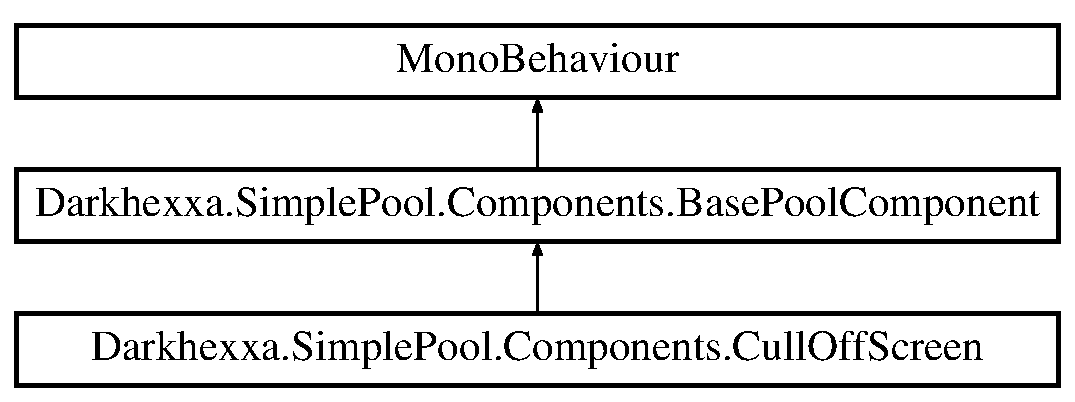
\includegraphics[height=3.000000cm]{class_darkhexxa_1_1_simple_pool_1_1_components_1_1_base_pool_component}
\end{center}
\end{figure}
\subsection*{Public Member Functions}
\begin{DoxyCompactItemize}
\item 
void \hyperlink{class_darkhexxa_1_1_simple_pool_1_1_components_1_1_base_pool_component_ad964a83becdd44af7ba763293d7f5e75}{On\-Created\-By\-Pool} (\hyperlink{class_darkhexxa_1_1_simple_pool_1_1_simple_pool}{Simple\-Pool} \hyperlink{class_darkhexxa_1_1_simple_pool_1_1_components_1_1_base_pool_component_a998b7d9d011951e36f93a020fe788022}{pool})
\item 
abstract void \hyperlink{class_darkhexxa_1_1_simple_pool_1_1_components_1_1_base_pool_component_a7173f329105a68229c0c4de3e08faf20}{On\-Spawn} ()
\item 
abstract void \hyperlink{class_darkhexxa_1_1_simple_pool_1_1_components_1_1_base_pool_component_a23947e638a808f92c5f4206ffcba8ec2}{On\-Despawn} ()
\end{DoxyCompactItemize}
\subsection*{Properties}
\begin{DoxyCompactItemize}
\item 
\hyperlink{class_darkhexxa_1_1_simple_pool_1_1_simple_pool}{Simple\-Pool} \hyperlink{class_darkhexxa_1_1_simple_pool_1_1_components_1_1_base_pool_component_a998b7d9d011951e36f93a020fe788022}{pool}\hspace{0.3cm}{\ttfamily  \mbox{[}get\mbox{]}}
\end{DoxyCompactItemize}


\subsection{Detailed Description}
Abstact Base class for Game\-Objects created by pools. 

Definition at line 24 of file Base\-Pool\-Component.\-cs.



\subsection{Member Function Documentation}
\hypertarget{class_darkhexxa_1_1_simple_pool_1_1_components_1_1_base_pool_component_ad964a83becdd44af7ba763293d7f5e75}{\index{Darkhexxa\-::\-Simple\-Pool\-::\-Components\-::\-Base\-Pool\-Component@{Darkhexxa\-::\-Simple\-Pool\-::\-Components\-::\-Base\-Pool\-Component}!On\-Created\-By\-Pool@{On\-Created\-By\-Pool}}
\index{On\-Created\-By\-Pool@{On\-Created\-By\-Pool}!Darkhexxa::SimplePool::Components::BasePoolComponent@{Darkhexxa\-::\-Simple\-Pool\-::\-Components\-::\-Base\-Pool\-Component}}
\subsubsection[{On\-Created\-By\-Pool}]{\setlength{\rightskip}{0pt plus 5cm}void Darkhexxa.\-Simple\-Pool.\-Components.\-Base\-Pool\-Component.\-On\-Created\-By\-Pool (
\begin{DoxyParamCaption}
\item[{{\bf Simple\-Pool}}]{pool}
\end{DoxyParamCaption}
)}}\label{class_darkhexxa_1_1_simple_pool_1_1_components_1_1_base_pool_component_ad964a83becdd44af7ba763293d7f5e75}
{\bfseries function} called by \hyperlink{class_darkhexxa_1_1_simple_pool_1_1_simple_pool}{Simple\-Pool} when an object is cloned.

Allows code to be implemented when this object is added to the scene but is not yet active.


\begin{DoxyParams}{Parameters}
{\em the} & simple pool that created this object. \\
\hline
\end{DoxyParams}


Definition at line 45 of file Base\-Pool\-Component.\-cs.

\hypertarget{class_darkhexxa_1_1_simple_pool_1_1_components_1_1_base_pool_component_a23947e638a808f92c5f4206ffcba8ec2}{\index{Darkhexxa\-::\-Simple\-Pool\-::\-Components\-::\-Base\-Pool\-Component@{Darkhexxa\-::\-Simple\-Pool\-::\-Components\-::\-Base\-Pool\-Component}!On\-Despawn@{On\-Despawn}}
\index{On\-Despawn@{On\-Despawn}!Darkhexxa::SimplePool::Components::BasePoolComponent@{Darkhexxa\-::\-Simple\-Pool\-::\-Components\-::\-Base\-Pool\-Component}}
\subsubsection[{On\-Despawn}]{\setlength{\rightskip}{0pt plus 5cm}abstract void Darkhexxa.\-Simple\-Pool.\-Components.\-Base\-Pool\-Component.\-On\-Despawn (
\begin{DoxyParamCaption}
{}
\end{DoxyParamCaption}
)\hspace{0.3cm}{\ttfamily [pure virtual]}}}\label{class_darkhexxa_1_1_simple_pool_1_1_components_1_1_base_pool_component_a23947e638a808f92c5f4206ffcba8ec2}
{\bfseries abstract} function that is called when the object is removed and becomes inactive. 

Implemented in \hyperlink{class_darkhexxa_1_1_simple_pool_1_1_components_1_1_cull_off_screen_a5f4a09e2cb31817af47ed394f4482bec}{Darkhexxa.\-Simple\-Pool.\-Components.\-Cull\-Off\-Screen}.

\hypertarget{class_darkhexxa_1_1_simple_pool_1_1_components_1_1_base_pool_component_a7173f329105a68229c0c4de3e08faf20}{\index{Darkhexxa\-::\-Simple\-Pool\-::\-Components\-::\-Base\-Pool\-Component@{Darkhexxa\-::\-Simple\-Pool\-::\-Components\-::\-Base\-Pool\-Component}!On\-Spawn@{On\-Spawn}}
\index{On\-Spawn@{On\-Spawn}!Darkhexxa::SimplePool::Components::BasePoolComponent@{Darkhexxa\-::\-Simple\-Pool\-::\-Components\-::\-Base\-Pool\-Component}}
\subsubsection[{On\-Spawn}]{\setlength{\rightskip}{0pt plus 5cm}abstract void Darkhexxa.\-Simple\-Pool.\-Components.\-Base\-Pool\-Component.\-On\-Spawn (
\begin{DoxyParamCaption}
{}
\end{DoxyParamCaption}
)\hspace{0.3cm}{\ttfamily [pure virtual]}}}\label{class_darkhexxa_1_1_simple_pool_1_1_components_1_1_base_pool_component_a7173f329105a68229c0c4de3e08faf20}
{\bfseries abstract} function that is called when the object is spawned and becomes active. 

Implemented in \hyperlink{class_darkhexxa_1_1_simple_pool_1_1_components_1_1_cull_off_screen_ad85eb1ac683e2368d1aa96c18bd9d317}{Darkhexxa.\-Simple\-Pool.\-Components.\-Cull\-Off\-Screen}.



\subsection{Property Documentation}
\hypertarget{class_darkhexxa_1_1_simple_pool_1_1_components_1_1_base_pool_component_a998b7d9d011951e36f93a020fe788022}{\index{Darkhexxa\-::\-Simple\-Pool\-::\-Components\-::\-Base\-Pool\-Component@{Darkhexxa\-::\-Simple\-Pool\-::\-Components\-::\-Base\-Pool\-Component}!pool@{pool}}
\index{pool@{pool}!Darkhexxa::SimplePool::Components::BasePoolComponent@{Darkhexxa\-::\-Simple\-Pool\-::\-Components\-::\-Base\-Pool\-Component}}
\subsubsection[{pool}]{\setlength{\rightskip}{0pt plus 5cm}{\bf Simple\-Pool} Darkhexxa.\-Simple\-Pool.\-Components.\-Base\-Pool\-Component.\-pool\hspace{0.3cm}{\ttfamily [get]}}}\label{class_darkhexxa_1_1_simple_pool_1_1_components_1_1_base_pool_component_a998b7d9d011951e36f93a020fe788022}
{\bfseries the} pool component that spawned this object. 

Definition at line 31 of file Base\-Pool\-Component.\-cs.



The documentation for this class was generated from the following file\-:\begin{DoxyCompactItemize}
\item 
C\-:/\-Users/\-Anthony/\-Game\-\_\-\-Development/\-Unity\-\_\-\-Projects/\-Darkhexxa/\-Assets/\-Darkhexxa/\-Simpel\-Pool/\-Components/\hyperlink{_base_pool_component_8cs}{Base\-Pool\-Component.\-cs}\end{DoxyCompactItemize}

\hypertarget{class_darkhexxa_1_1_core_1_1_component_list}{\section{Darkhexxa.\-Core.\-Component\-List Class Reference}
\label{class_darkhexxa_1_1_core_1_1_component_list}\index{Darkhexxa.\-Core.\-Component\-List@{Darkhexxa.\-Core.\-Component\-List}}
}
\subsection*{Public Member Functions}
\begin{DoxyCompactItemize}
\item 
\hyperlink{class_darkhexxa_1_1_core_1_1_component_list_a0a28059a3c3d8ace2f0a789ebca9fe9a}{Component\-List} ()
\item 
void \hyperlink{class_darkhexxa_1_1_core_1_1_component_list_a38227b1b1c70988750d8b9faeb8109b9}{Insert\-At\-Head} (ref Game\-Object obj)
\item 
void \hyperlink{class_darkhexxa_1_1_core_1_1_component_list_a74ba809eec19ce341cc5d8c685eaea5b}{Insert\-At\-Tail} (ref Game\-Object obj)
\item 
Game\-Object \hyperlink{class_darkhexxa_1_1_core_1_1_component_list_a4baff132dc5c3de864a6b2e30a6a3212}{Remove\-Head\-G\-O} ()
\item 
Game\-Object \hyperlink{class_darkhexxa_1_1_core_1_1_component_list_a80ab55bc996e84f373fedceeb188f76e}{Remove\-Tail\-G\-O} ()
\item 
void \hyperlink{class_darkhexxa_1_1_core_1_1_component_list_a47f636d5d6dc55dabb3e832de5fe2569}{Remove} (Game\-Object obj)
\end{DoxyCompactItemize}
\subsection*{Properties}
\begin{DoxyCompactItemize}
\item 
\hyperlink{class_darkhexxa_1_1_core_1_1_listable_component}{Listable\-Component} \hyperlink{class_darkhexxa_1_1_core_1_1_component_list_aaf3c579fbb8e52b3077d38dd218ec357}{Head}\hspace{0.3cm}{\ttfamily  \mbox{[}get\mbox{]}}
\begin{DoxyCompactList}\small\item\em number of items in the list \end{DoxyCompactList}\item 
\hyperlink{class_darkhexxa_1_1_core_1_1_listable_component}{Listable\-Component} \hyperlink{class_darkhexxa_1_1_core_1_1_component_list_a5690588d6657c520569aa5cd171914ea}{Tail}\hspace{0.3cm}{\ttfamily  \mbox{[}get\mbox{]}}
\item 
int \hyperlink{class_darkhexxa_1_1_core_1_1_component_list_acc444401550cdd597358ef21bd527404}{Count}\hspace{0.3cm}{\ttfamily  \mbox{[}get\mbox{]}}
\item 
bool \hyperlink{class_darkhexxa_1_1_core_1_1_component_list_a7566c88897f93bb027480738d184907b}{is\-Empty}\hspace{0.3cm}{\ttfamily  \mbox{[}get\mbox{]}}
\end{DoxyCompactItemize}


\subsection{Detailed Description}


Definition at line 22 of file Component\-List.\-cs.



\subsection{Constructor \& Destructor Documentation}
\hypertarget{class_darkhexxa_1_1_core_1_1_component_list_a0a28059a3c3d8ace2f0a789ebca9fe9a}{\index{Darkhexxa\-::\-Core\-::\-Component\-List@{Darkhexxa\-::\-Core\-::\-Component\-List}!Component\-List@{Component\-List}}
\index{Component\-List@{Component\-List}!Darkhexxa::Core::ComponentList@{Darkhexxa\-::\-Core\-::\-Component\-List}}
\subsubsection[{Component\-List}]{\setlength{\rightskip}{0pt plus 5cm}Darkhexxa.\-Core.\-Component\-List.\-Component\-List (
\begin{DoxyParamCaption}
{}
\end{DoxyParamCaption}
)}}\label{class_darkhexxa_1_1_core_1_1_component_list_a0a28059a3c3d8ace2f0a789ebca9fe9a}


Definition at line 47 of file Component\-List.\-cs.



\subsection{Member Function Documentation}
\hypertarget{class_darkhexxa_1_1_core_1_1_component_list_a38227b1b1c70988750d8b9faeb8109b9}{\index{Darkhexxa\-::\-Core\-::\-Component\-List@{Darkhexxa\-::\-Core\-::\-Component\-List}!Insert\-At\-Head@{Insert\-At\-Head}}
\index{Insert\-At\-Head@{Insert\-At\-Head}!Darkhexxa::Core::ComponentList@{Darkhexxa\-::\-Core\-::\-Component\-List}}
\subsubsection[{Insert\-At\-Head}]{\setlength{\rightskip}{0pt plus 5cm}void Darkhexxa.\-Core.\-Component\-List.\-Insert\-At\-Head (
\begin{DoxyParamCaption}
\item[{ref Game\-Object}]{obj}
\end{DoxyParamCaption}
)}}\label{class_darkhexxa_1_1_core_1_1_component_list_a38227b1b1c70988750d8b9faeb8109b9}


Definition at line 72 of file Component\-List.\-cs.

\hypertarget{class_darkhexxa_1_1_core_1_1_component_list_a74ba809eec19ce341cc5d8c685eaea5b}{\index{Darkhexxa\-::\-Core\-::\-Component\-List@{Darkhexxa\-::\-Core\-::\-Component\-List}!Insert\-At\-Tail@{Insert\-At\-Tail}}
\index{Insert\-At\-Tail@{Insert\-At\-Tail}!Darkhexxa::Core::ComponentList@{Darkhexxa\-::\-Core\-::\-Component\-List}}
\subsubsection[{Insert\-At\-Tail}]{\setlength{\rightskip}{0pt plus 5cm}void Darkhexxa.\-Core.\-Component\-List.\-Insert\-At\-Tail (
\begin{DoxyParamCaption}
\item[{ref Game\-Object}]{obj}
\end{DoxyParamCaption}
)}}\label{class_darkhexxa_1_1_core_1_1_component_list_a74ba809eec19ce341cc5d8c685eaea5b}


Definition at line 97 of file Component\-List.\-cs.

\hypertarget{class_darkhexxa_1_1_core_1_1_component_list_a47f636d5d6dc55dabb3e832de5fe2569}{\index{Darkhexxa\-::\-Core\-::\-Component\-List@{Darkhexxa\-::\-Core\-::\-Component\-List}!Remove@{Remove}}
\index{Remove@{Remove}!Darkhexxa::Core::ComponentList@{Darkhexxa\-::\-Core\-::\-Component\-List}}
\subsubsection[{Remove}]{\setlength{\rightskip}{0pt plus 5cm}void Darkhexxa.\-Core.\-Component\-List.\-Remove (
\begin{DoxyParamCaption}
\item[{Game\-Object}]{obj}
\end{DoxyParamCaption}
)}}\label{class_darkhexxa_1_1_core_1_1_component_list_a47f636d5d6dc55dabb3e832de5fe2569}


Definition at line 210 of file Component\-List.\-cs.

\hypertarget{class_darkhexxa_1_1_core_1_1_component_list_a4baff132dc5c3de864a6b2e30a6a3212}{\index{Darkhexxa\-::\-Core\-::\-Component\-List@{Darkhexxa\-::\-Core\-::\-Component\-List}!Remove\-Head\-G\-O@{Remove\-Head\-G\-O}}
\index{Remove\-Head\-G\-O@{Remove\-Head\-G\-O}!Darkhexxa::Core::ComponentList@{Darkhexxa\-::\-Core\-::\-Component\-List}}
\subsubsection[{Remove\-Head\-G\-O}]{\setlength{\rightskip}{0pt plus 5cm}Game\-Object Darkhexxa.\-Core.\-Component\-List.\-Remove\-Head\-G\-O (
\begin{DoxyParamCaption}
{}
\end{DoxyParamCaption}
)}}\label{class_darkhexxa_1_1_core_1_1_component_list_a4baff132dc5c3de864a6b2e30a6a3212}


Definition at line 117 of file Component\-List.\-cs.

\hypertarget{class_darkhexxa_1_1_core_1_1_component_list_a80ab55bc996e84f373fedceeb188f76e}{\index{Darkhexxa\-::\-Core\-::\-Component\-List@{Darkhexxa\-::\-Core\-::\-Component\-List}!Remove\-Tail\-G\-O@{Remove\-Tail\-G\-O}}
\index{Remove\-Tail\-G\-O@{Remove\-Tail\-G\-O}!Darkhexxa::Core::ComponentList@{Darkhexxa\-::\-Core\-::\-Component\-List}}
\subsubsection[{Remove\-Tail\-G\-O}]{\setlength{\rightskip}{0pt plus 5cm}Game\-Object Darkhexxa.\-Core.\-Component\-List.\-Remove\-Tail\-G\-O (
\begin{DoxyParamCaption}
{}
\end{DoxyParamCaption}
)}}\label{class_darkhexxa_1_1_core_1_1_component_list_a80ab55bc996e84f373fedceeb188f76e}


Definition at line 137 of file Component\-List.\-cs.



\subsection{Property Documentation}
\hypertarget{class_darkhexxa_1_1_core_1_1_component_list_acc444401550cdd597358ef21bd527404}{\index{Darkhexxa\-::\-Core\-::\-Component\-List@{Darkhexxa\-::\-Core\-::\-Component\-List}!Count@{Count}}
\index{Count@{Count}!Darkhexxa::Core::ComponentList@{Darkhexxa\-::\-Core\-::\-Component\-List}}
\subsubsection[{Count}]{\setlength{\rightskip}{0pt plus 5cm}int Darkhexxa.\-Core.\-Component\-List.\-Count\hspace{0.3cm}{\ttfamily [get]}}}\label{class_darkhexxa_1_1_core_1_1_component_list_acc444401550cdd597358ef21bd527404}


Definition at line 32 of file Component\-List.\-cs.

\hypertarget{class_darkhexxa_1_1_core_1_1_component_list_aaf3c579fbb8e52b3077d38dd218ec357}{\index{Darkhexxa\-::\-Core\-::\-Component\-List@{Darkhexxa\-::\-Core\-::\-Component\-List}!Head@{Head}}
\index{Head@{Head}!Darkhexxa::Core::ComponentList@{Darkhexxa\-::\-Core\-::\-Component\-List}}
\subsubsection[{Head}]{\setlength{\rightskip}{0pt plus 5cm}{\bf Listable\-Component} Darkhexxa.\-Core.\-Component\-List.\-Head\hspace{0.3cm}{\ttfamily [get]}}}\label{class_darkhexxa_1_1_core_1_1_component_list_aaf3c579fbb8e52b3077d38dd218ec357}


number of items in the list 



Definition at line 28 of file Component\-List.\-cs.

\hypertarget{class_darkhexxa_1_1_core_1_1_component_list_a7566c88897f93bb027480738d184907b}{\index{Darkhexxa\-::\-Core\-::\-Component\-List@{Darkhexxa\-::\-Core\-::\-Component\-List}!is\-Empty@{is\-Empty}}
\index{is\-Empty@{is\-Empty}!Darkhexxa::Core::ComponentList@{Darkhexxa\-::\-Core\-::\-Component\-List}}
\subsubsection[{is\-Empty}]{\setlength{\rightskip}{0pt plus 5cm}bool Darkhexxa.\-Core.\-Component\-List.\-is\-Empty\hspace{0.3cm}{\ttfamily [get]}}}\label{class_darkhexxa_1_1_core_1_1_component_list_a7566c88897f93bb027480738d184907b}


Definition at line 40 of file Component\-List.\-cs.

\hypertarget{class_darkhexxa_1_1_core_1_1_component_list_a5690588d6657c520569aa5cd171914ea}{\index{Darkhexxa\-::\-Core\-::\-Component\-List@{Darkhexxa\-::\-Core\-::\-Component\-List}!Tail@{Tail}}
\index{Tail@{Tail}!Darkhexxa::Core::ComponentList@{Darkhexxa\-::\-Core\-::\-Component\-List}}
\subsubsection[{Tail}]{\setlength{\rightskip}{0pt plus 5cm}{\bf Listable\-Component} Darkhexxa.\-Core.\-Component\-List.\-Tail\hspace{0.3cm}{\ttfamily [get]}}}\label{class_darkhexxa_1_1_core_1_1_component_list_a5690588d6657c520569aa5cd171914ea}


Definition at line 29 of file Component\-List.\-cs.



The documentation for this class was generated from the following file\-:\begin{DoxyCompactItemize}
\item 
C\-:/\-Users/\-Anthony/\-Game\-\_\-\-Development/\-Unity\-\_\-\-Projects/\-Darkhexxa/\-Assets/\-Darkhexxa/\-Core/\hyperlink{_component_list_8cs}{Component\-List.\-cs}\end{DoxyCompactItemize}

\hypertarget{class_darkhexxa_1_1_simple_pool_1_1_components_1_1_cull_off_screen}{\section{Darkhexxa.\-Simple\-Pool.\-Components.\-Cull\-Off\-Screen Class Reference}
\label{class_darkhexxa_1_1_simple_pool_1_1_components_1_1_cull_off_screen}\index{Darkhexxa.\-Simple\-Pool.\-Components.\-Cull\-Off\-Screen@{Darkhexxa.\-Simple\-Pool.\-Components.\-Cull\-Off\-Screen}}
}


A base pool component that despawns the attached object when it goes off screen.  


Inheritance diagram for Darkhexxa.\-Simple\-Pool.\-Components.\-Cull\-Off\-Screen\-:\begin{figure}[H]
\begin{center}
\leavevmode
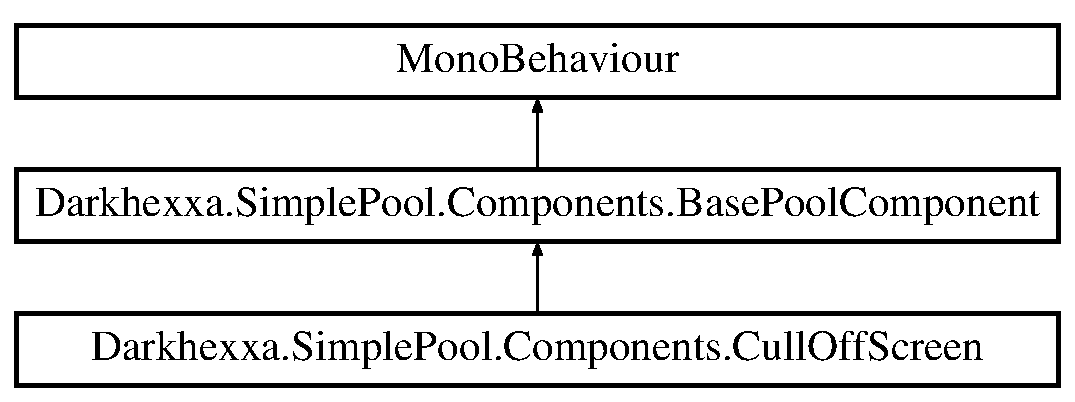
\includegraphics[height=3.000000cm]{class_darkhexxa_1_1_simple_pool_1_1_components_1_1_cull_off_screen}
\end{center}
\end{figure}
\subsection*{Public Member Functions}
\begin{DoxyCompactItemize}
\item 
override void \hyperlink{class_darkhexxa_1_1_simple_pool_1_1_components_1_1_cull_off_screen_ad85eb1ac683e2368d1aa96c18bd9d317}{On\-Spawn} ()
\item 
override void \hyperlink{class_darkhexxa_1_1_simple_pool_1_1_components_1_1_cull_off_screen_a5f4a09e2cb31817af47ed394f4482bec}{On\-Despawn} ()
\end{DoxyCompactItemize}
\subsection*{Additional Inherited Members}


\subsection{Detailed Description}
A base pool component that despawns the attached object when it goes off screen. 

Definition at line 15 of file Cull\-Off\-Screen.\-cs.



\subsection{Member Function Documentation}
\hypertarget{class_darkhexxa_1_1_simple_pool_1_1_components_1_1_cull_off_screen_a5f4a09e2cb31817af47ed394f4482bec}{\index{Darkhexxa\-::\-Simple\-Pool\-::\-Components\-::\-Cull\-Off\-Screen@{Darkhexxa\-::\-Simple\-Pool\-::\-Components\-::\-Cull\-Off\-Screen}!On\-Despawn@{On\-Despawn}}
\index{On\-Despawn@{On\-Despawn}!Darkhexxa::SimplePool::Components::CullOffScreen@{Darkhexxa\-::\-Simple\-Pool\-::\-Components\-::\-Cull\-Off\-Screen}}
\subsubsection[{On\-Despawn}]{\setlength{\rightskip}{0pt plus 5cm}override void Darkhexxa.\-Simple\-Pool.\-Components.\-Cull\-Off\-Screen.\-On\-Despawn (
\begin{DoxyParamCaption}
{}
\end{DoxyParamCaption}
)\hspace{0.3cm}{\ttfamily [virtual]}}}\label{class_darkhexxa_1_1_simple_pool_1_1_components_1_1_cull_off_screen_a5f4a09e2cb31817af47ed394f4482bec}
{\bfseries abstract} function that is called when the object is removed and becomes inactive. 

Implements \hyperlink{class_darkhexxa_1_1_simple_pool_1_1_components_1_1_base_pool_component_a23947e638a808f92c5f4206ffcba8ec2}{Darkhexxa.\-Simple\-Pool.\-Components.\-Base\-Pool\-Component}.



Definition at line 22 of file Cull\-Off\-Screen.\-cs.

\hypertarget{class_darkhexxa_1_1_simple_pool_1_1_components_1_1_cull_off_screen_ad85eb1ac683e2368d1aa96c18bd9d317}{\index{Darkhexxa\-::\-Simple\-Pool\-::\-Components\-::\-Cull\-Off\-Screen@{Darkhexxa\-::\-Simple\-Pool\-::\-Components\-::\-Cull\-Off\-Screen}!On\-Spawn@{On\-Spawn}}
\index{On\-Spawn@{On\-Spawn}!Darkhexxa::SimplePool::Components::CullOffScreen@{Darkhexxa\-::\-Simple\-Pool\-::\-Components\-::\-Cull\-Off\-Screen}}
\subsubsection[{On\-Spawn}]{\setlength{\rightskip}{0pt plus 5cm}override void Darkhexxa.\-Simple\-Pool.\-Components.\-Cull\-Off\-Screen.\-On\-Spawn (
\begin{DoxyParamCaption}
{}
\end{DoxyParamCaption}
)\hspace{0.3cm}{\ttfamily [virtual]}}}\label{class_darkhexxa_1_1_simple_pool_1_1_components_1_1_cull_off_screen_ad85eb1ac683e2368d1aa96c18bd9d317}
{\bfseries abstract} function that is called when the object is spawned and becomes active. 

Implements \hyperlink{class_darkhexxa_1_1_simple_pool_1_1_components_1_1_base_pool_component_a7173f329105a68229c0c4de3e08faf20}{Darkhexxa.\-Simple\-Pool.\-Components.\-Base\-Pool\-Component}.



Definition at line 18 of file Cull\-Off\-Screen.\-cs.



The documentation for this class was generated from the following file\-:\begin{DoxyCompactItemize}
\item 
C\-:/\-Users/\-Anthony/\-Game\-\_\-\-Development/\-Unity\-\_\-\-Projects/\-Darkhexxa/\-Assets/\-Darkhexxa/\-Simpel\-Pool/\-Components/\hyperlink{_cull_off_screen_8cs}{Cull\-Off\-Screen.\-cs}\end{DoxyCompactItemize}

\hypertarget{class_darkhexxa_1_1_core_1_1_listable_component}{\section{Darkhexxa.\-Core.\-Listable\-Component Class Reference}
\label{class_darkhexxa_1_1_core_1_1_listable_component}\index{Darkhexxa.\-Core.\-Listable\-Component@{Darkhexxa.\-Core.\-Listable\-Component}}
}
Inheritance diagram for Darkhexxa.\-Core.\-Listable\-Component\-:\begin{figure}[H]
\begin{center}
\leavevmode
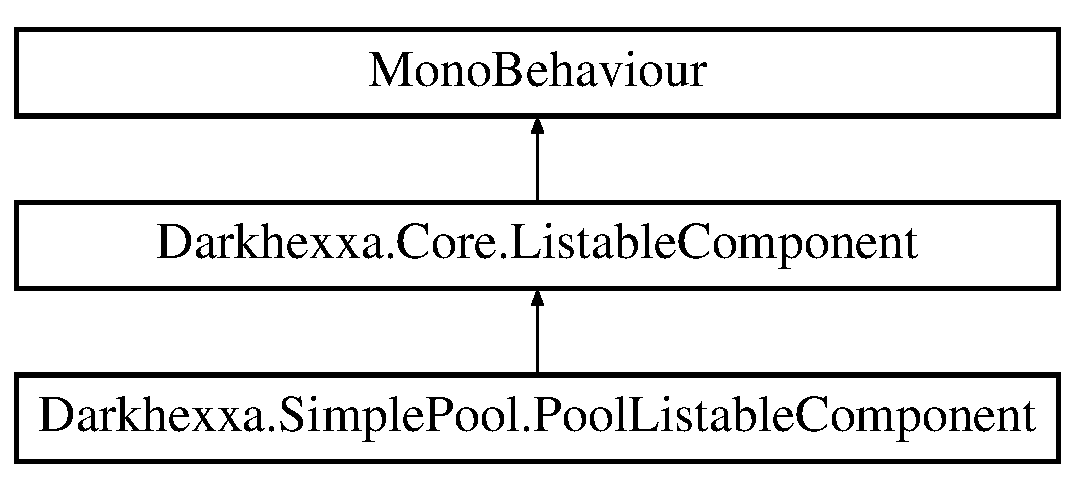
\includegraphics[height=3.000000cm]{class_darkhexxa_1_1_core_1_1_listable_component}
\end{center}
\end{figure}
\subsection*{Properties}
\begin{DoxyCompactItemize}
\item 
\hyperlink{class_darkhexxa_1_1_core_1_1_component_list}{Component\-List} \hyperlink{class_darkhexxa_1_1_core_1_1_listable_component_a04c51fde5d01ceae927e191e1420c27e}{list}\hspace{0.3cm}{\ttfamily  \mbox{[}get, set\mbox{]}}
\item 
\hyperlink{class_darkhexxa_1_1_core_1_1_listable_component}{Listable\-Component} \hyperlink{class_darkhexxa_1_1_core_1_1_listable_component_afe73beef049d8199b6c205e27653ae29}{Previous}\hspace{0.3cm}{\ttfamily  \mbox{[}get, set\mbox{]}}
\item 
\hyperlink{class_darkhexxa_1_1_core_1_1_listable_component}{Listable\-Component} \hyperlink{class_darkhexxa_1_1_core_1_1_listable_component_acd3a93b2ac0c5536bad8a3fd74cc1e5a}{Next}\hspace{0.3cm}{\ttfamily  \mbox{[}get, set\mbox{]}}
\end{DoxyCompactItemize}


\subsection{Detailed Description}


Definition at line 18 of file Listable\-Component.\-cs.



\subsection{Property Documentation}
\hypertarget{class_darkhexxa_1_1_core_1_1_listable_component_a04c51fde5d01ceae927e191e1420c27e}{\index{Darkhexxa\-::\-Core\-::\-Listable\-Component@{Darkhexxa\-::\-Core\-::\-Listable\-Component}!list@{list}}
\index{list@{list}!Darkhexxa::Core::ListableComponent@{Darkhexxa\-::\-Core\-::\-Listable\-Component}}
\subsubsection[{list}]{\setlength{\rightskip}{0pt plus 5cm}{\bf Component\-List} Darkhexxa.\-Core.\-Listable\-Component.\-list\hspace{0.3cm}{\ttfamily [get]}, {\ttfamily [set]}}}\label{class_darkhexxa_1_1_core_1_1_listable_component_a04c51fde5d01ceae927e191e1420c27e}


Definition at line 27 of file Listable\-Component.\-cs.

\hypertarget{class_darkhexxa_1_1_core_1_1_listable_component_acd3a93b2ac0c5536bad8a3fd74cc1e5a}{\index{Darkhexxa\-::\-Core\-::\-Listable\-Component@{Darkhexxa\-::\-Core\-::\-Listable\-Component}!Next@{Next}}
\index{Next@{Next}!Darkhexxa::Core::ListableComponent@{Darkhexxa\-::\-Core\-::\-Listable\-Component}}
\subsubsection[{Next}]{\setlength{\rightskip}{0pt plus 5cm}{\bf Listable\-Component} Darkhexxa.\-Core.\-Listable\-Component.\-Next\hspace{0.3cm}{\ttfamily [get]}, {\ttfamily [set]}}}\label{class_darkhexxa_1_1_core_1_1_listable_component_acd3a93b2ac0c5536bad8a3fd74cc1e5a}


Definition at line 51 of file Listable\-Component.\-cs.

\hypertarget{class_darkhexxa_1_1_core_1_1_listable_component_afe73beef049d8199b6c205e27653ae29}{\index{Darkhexxa\-::\-Core\-::\-Listable\-Component@{Darkhexxa\-::\-Core\-::\-Listable\-Component}!Previous@{Previous}}
\index{Previous@{Previous}!Darkhexxa::Core::ListableComponent@{Darkhexxa\-::\-Core\-::\-Listable\-Component}}
\subsubsection[{Previous}]{\setlength{\rightskip}{0pt plus 5cm}{\bf Listable\-Component} Darkhexxa.\-Core.\-Listable\-Component.\-Previous\hspace{0.3cm}{\ttfamily [get]}, {\ttfamily [set]}}}\label{class_darkhexxa_1_1_core_1_1_listable_component_afe73beef049d8199b6c205e27653ae29}


Definition at line 39 of file Listable\-Component.\-cs.



The documentation for this class was generated from the following file\-:\begin{DoxyCompactItemize}
\item 
C\-:/\-Users/\-Anthony/\-Game\-\_\-\-Development/\-Unity\-\_\-\-Projects/\-Darkhexxa/\-Assets/\-Darkhexxa/\-Core/\hyperlink{_listable_component_8cs}{Listable\-Component.\-cs}\end{DoxyCompactItemize}

\hypertarget{class_darkhexxa_1_1_simple_pool_1_1_simple_pool_1_1_pool_data}{\section{Darkhexxa.\-Simple\-Pool.\-Simple\-Pool.\-Pool\-Data Class Reference}
\label{class_darkhexxa_1_1_simple_pool_1_1_simple_pool_1_1_pool_data}\index{Darkhexxa.\-Simple\-Pool.\-Simple\-Pool.\-Pool\-Data@{Darkhexxa.\-Simple\-Pool.\-Simple\-Pool.\-Pool\-Data}}
}


Data for the pool.  


\subsection*{Public Member Functions}
\begin{DoxyCompactItemize}
\item 
\hyperlink{class_darkhexxa_1_1_simple_pool_1_1_simple_pool_1_1_pool_data_a362fa5c969fb8230d2248dd6d8590b65}{Pool\-Data} (Game\-Object \hyperlink{class_darkhexxa_1_1_simple_pool_1_1_simple_pool_1_1_pool_data_afeeca245f87b8bef8c5a954c7b78011c}{prefab})
\begin{DoxyCompactList}\small\item\em \begin{quotation}
the interval for the calling process. \end{quotation}
\end{DoxyCompactList}\item 
\hyperlink{class_darkhexxa_1_1_simple_pool_1_1_simple_pool_1_1_pool_data_a0b538556ad116b32f300845651d86a30}{Pool\-Data} (Game\-Object \hyperlink{class_darkhexxa_1_1_simple_pool_1_1_simple_pool_1_1_pool_data_afeeca245f87b8bef8c5a954c7b78011c}{prefab}, int \hyperlink{class_darkhexxa_1_1_simple_pool_1_1_simple_pool_1_1_pool_data_ae2d66b8c6f3d77721c5ca3474cac1311}{max\-Count}, int \hyperlink{class_darkhexxa_1_1_simple_pool_1_1_simple_pool_1_1_pool_data_a7277e7f63a6189198b789f74db585a94}{batch\-Create\-Count}, bool \hyperlink{class_darkhexxa_1_1_simple_pool_1_1_simple_pool_1_1_pool_data_a19c48ea469a33d4188a996482939d665}{cull\-Inactive}, float \hyperlink{class_darkhexxa_1_1_simple_pool_1_1_simple_pool_1_1_pool_data_abf0fe104db5c39105f7c88dca1581bc1}{cull\-Interval})
\item 
override bool \hyperlink{class_darkhexxa_1_1_simple_pool_1_1_simple_pool_1_1_pool_data_a3b57abc0a9ad8594aba92e4987869e72}{Equals} (object obj)
\item 
override int \hyperlink{class_darkhexxa_1_1_simple_pool_1_1_simple_pool_1_1_pool_data_ac38a6df31961bb203a80c01d5d4b855c}{Get\-Hash\-Code} ()
\end{DoxyCompactItemize}
\subsection*{Static Public Member Functions}
\begin{DoxyCompactItemize}
\item 
static bool \hyperlink{class_darkhexxa_1_1_simple_pool_1_1_simple_pool_1_1_pool_data_a2ec19cce5e6f1b26aa952c5301b98fef}{operator==} (\hyperlink{class_darkhexxa_1_1_simple_pool_1_1_simple_pool_1_1_pool_data}{Pool\-Data} data1, \hyperlink{class_darkhexxa_1_1_simple_pool_1_1_simple_pool_1_1_pool_data}{Pool\-Data} data2)
\item 
static bool \hyperlink{class_darkhexxa_1_1_simple_pool_1_1_simple_pool_1_1_pool_data_addc62fa3d584aa771c25dcefa4a18986}{operator!=} (\hyperlink{class_darkhexxa_1_1_simple_pool_1_1_simple_pool_1_1_pool_data}{Pool\-Data} data1, \hyperlink{class_darkhexxa_1_1_simple_pool_1_1_simple_pool_1_1_pool_data}{Pool\-Data} data2)
\end{DoxyCompactItemize}
\subsection*{Public Attributes}
\begin{DoxyCompactItemize}
\item 
Game\-Object \hyperlink{class_darkhexxa_1_1_simple_pool_1_1_simple_pool_1_1_pool_data_afeeca245f87b8bef8c5a954c7b78011c}{prefab}
\item 
int \hyperlink{class_darkhexxa_1_1_simple_pool_1_1_simple_pool_1_1_pool_data_ae2d66b8c6f3d77721c5ca3474cac1311}{max\-Count} = 0
\begin{DoxyCompactList}\small\item\em \begin{quotation}
game object to clone \end{quotation}
\end{DoxyCompactList}\item 
int \hyperlink{class_darkhexxa_1_1_simple_pool_1_1_simple_pool_1_1_pool_data_a7277e7f63a6189198b789f74db585a94}{batch\-Create\-Count} = 5
\begin{DoxyCompactList}\small\item\em \begin{quotation}
max number of clones \end{quotation}
\end{DoxyCompactList}\item 
bool \hyperlink{class_darkhexxa_1_1_simple_pool_1_1_simple_pool_1_1_pool_data_a19c48ea469a33d4188a996482939d665}{cull\-Inactive} = false
\begin{DoxyCompactList}\small\item\em \begin{quotation}
number of clones to create when new objects are needed. \end{quotation}
\end{DoxyCompactList}\item 
float \hyperlink{class_darkhexxa_1_1_simple_pool_1_1_simple_pool_1_1_pool_data_abf0fe104db5c39105f7c88dca1581bc1}{cull\-Interval} = 10f
\begin{DoxyCompactList}\small\item\em \begin{quotation}
if culling of incactive objects is desired. \end{quotation}
\end{DoxyCompactList}\end{DoxyCompactItemize}


\subsection{Detailed Description}
Data for the pool. 

Definition at line 23 of file Simple\-Pool.\-cs.



\subsection{Constructor \& Destructor Documentation}
\hypertarget{class_darkhexxa_1_1_simple_pool_1_1_simple_pool_1_1_pool_data_a362fa5c969fb8230d2248dd6d8590b65}{\index{Darkhexxa\-::\-Simple\-Pool\-::\-Simple\-Pool\-::\-Pool\-Data@{Darkhexxa\-::\-Simple\-Pool\-::\-Simple\-Pool\-::\-Pool\-Data}!Pool\-Data@{Pool\-Data}}
\index{Pool\-Data@{Pool\-Data}!Darkhexxa::SimplePool::SimplePool::PoolData@{Darkhexxa\-::\-Simple\-Pool\-::\-Simple\-Pool\-::\-Pool\-Data}}
\subsubsection[{Pool\-Data}]{\setlength{\rightskip}{0pt plus 5cm}Darkhexxa.\-Simple\-Pool.\-Simple\-Pool.\-Pool\-Data.\-Pool\-Data (
\begin{DoxyParamCaption}
\item[{Game\-Object}]{prefab}
\end{DoxyParamCaption}
)}}\label{class_darkhexxa_1_1_simple_pool_1_1_simple_pool_1_1_pool_data_a362fa5c969fb8230d2248dd6d8590b65}


\begin{quotation}
the interval for the calling process. \end{quotation}


Constructor for \hyperlink{class_darkhexxa_1_1_simple_pool_1_1_simple_pool_1_1_pool_data}{Pool\-Data}


\begin{DoxyParams}{Parameters}
{\em Game\-Object} & to be cloned \\
\hline
\end{DoxyParams}


Definition at line 36 of file Simple\-Pool.\-cs.

\hypertarget{class_darkhexxa_1_1_simple_pool_1_1_simple_pool_1_1_pool_data_a0b538556ad116b32f300845651d86a30}{\index{Darkhexxa\-::\-Simple\-Pool\-::\-Simple\-Pool\-::\-Pool\-Data@{Darkhexxa\-::\-Simple\-Pool\-::\-Simple\-Pool\-::\-Pool\-Data}!Pool\-Data@{Pool\-Data}}
\index{Pool\-Data@{Pool\-Data}!Darkhexxa::SimplePool::SimplePool::PoolData@{Darkhexxa\-::\-Simple\-Pool\-::\-Simple\-Pool\-::\-Pool\-Data}}
\subsubsection[{Pool\-Data}]{\setlength{\rightskip}{0pt plus 5cm}Darkhexxa.\-Simple\-Pool.\-Simple\-Pool.\-Pool\-Data.\-Pool\-Data (
\begin{DoxyParamCaption}
\item[{Game\-Object}]{prefab, }
\item[{int}]{max\-Count, }
\item[{int}]{batch\-Create\-Count, }
\item[{bool}]{cull\-Inactive, }
\item[{float}]{cull\-Interval}
\end{DoxyParamCaption}
)}}\label{class_darkhexxa_1_1_simple_pool_1_1_simple_pool_1_1_pool_data_a0b538556ad116b32f300845651d86a30}
Constructor for \hyperlink{class_darkhexxa_1_1_simple_pool_1_1_simple_pool_1_1_pool_data}{Pool\-Data}


\begin{DoxyParams}{Parameters}
{\em Game\-Object} & to be cloned \\
\hline
{\em int} & max\-Count clone \\
\hline
{\em int} & batch\-Create\-Count to clone when new objects are required \\
\hline
{\em bool} & cull inactive objects \\
\hline
{\em float} & the cull interval \\
\hline
\end{DoxyParams}


Definition at line 54 of file Simple\-Pool.\-cs.



\subsection{Member Function Documentation}
\hypertarget{class_darkhexxa_1_1_simple_pool_1_1_simple_pool_1_1_pool_data_a3b57abc0a9ad8594aba92e4987869e72}{\index{Darkhexxa\-::\-Simple\-Pool\-::\-Simple\-Pool\-::\-Pool\-Data@{Darkhexxa\-::\-Simple\-Pool\-::\-Simple\-Pool\-::\-Pool\-Data}!Equals@{Equals}}
\index{Equals@{Equals}!Darkhexxa::SimplePool::SimplePool::PoolData@{Darkhexxa\-::\-Simple\-Pool\-::\-Simple\-Pool\-::\-Pool\-Data}}
\subsubsection[{Equals}]{\setlength{\rightskip}{0pt plus 5cm}override bool Darkhexxa.\-Simple\-Pool.\-Simple\-Pool.\-Pool\-Data.\-Equals (
\begin{DoxyParamCaption}
\item[{object}]{obj}
\end{DoxyParamCaption}
)}}\label{class_darkhexxa_1_1_simple_pool_1_1_simple_pool_1_1_pool_data_a3b57abc0a9ad8594aba92e4987869e72}
Equals override


\begin{DoxyParams}{Parameters}
{\em \hyperlink{class_darkhexxa_1_1_simple_pool_1_1_simple_pool_1_1_pool_data}{Pool\-Data}} & object \\
\hline
\end{DoxyParams}
\begin{DoxyReturn}{Returns}
true if objects are equal. 
\end{DoxyReturn}


Definition at line 82 of file Simple\-Pool.\-cs.

\hypertarget{class_darkhexxa_1_1_simple_pool_1_1_simple_pool_1_1_pool_data_ac38a6df31961bb203a80c01d5d4b855c}{\index{Darkhexxa\-::\-Simple\-Pool\-::\-Simple\-Pool\-::\-Pool\-Data@{Darkhexxa\-::\-Simple\-Pool\-::\-Simple\-Pool\-::\-Pool\-Data}!Get\-Hash\-Code@{Get\-Hash\-Code}}
\index{Get\-Hash\-Code@{Get\-Hash\-Code}!Darkhexxa::SimplePool::SimplePool::PoolData@{Darkhexxa\-::\-Simple\-Pool\-::\-Simple\-Pool\-::\-Pool\-Data}}
\subsubsection[{Get\-Hash\-Code}]{\setlength{\rightskip}{0pt plus 5cm}override int Darkhexxa.\-Simple\-Pool.\-Simple\-Pool.\-Pool\-Data.\-Get\-Hash\-Code (
\begin{DoxyParamCaption}
{}
\end{DoxyParamCaption}
)}}\label{class_darkhexxa_1_1_simple_pool_1_1_simple_pool_1_1_pool_data_ac38a6df31961bb203a80c01d5d4b855c}
generate hash code

\begin{DoxyReturn}{Returns}
int hashcode. 
\end{DoxyReturn}


Definition at line 107 of file Simple\-Pool.\-cs.

\hypertarget{class_darkhexxa_1_1_simple_pool_1_1_simple_pool_1_1_pool_data_addc62fa3d584aa771c25dcefa4a18986}{\index{Darkhexxa\-::\-Simple\-Pool\-::\-Simple\-Pool\-::\-Pool\-Data@{Darkhexxa\-::\-Simple\-Pool\-::\-Simple\-Pool\-::\-Pool\-Data}!operator!=@{operator!=}}
\index{operator!=@{operator!=}!Darkhexxa::SimplePool::SimplePool::PoolData@{Darkhexxa\-::\-Simple\-Pool\-::\-Simple\-Pool\-::\-Pool\-Data}}
\subsubsection[{operator!=}]{\setlength{\rightskip}{0pt plus 5cm}static bool Darkhexxa.\-Simple\-Pool.\-Simple\-Pool.\-Pool\-Data.\-operator!= (
\begin{DoxyParamCaption}
\item[{{\bf Pool\-Data}}]{data1, }
\item[{{\bf Pool\-Data}}]{data2}
\end{DoxyParamCaption}
)\hspace{0.3cm}{\ttfamily [static]}}}\label{class_darkhexxa_1_1_simple_pool_1_1_simple_pool_1_1_pool_data_addc62fa3d584aa771c25dcefa4a18986}
is not equal to operator


\begin{DoxyParams}{Parameters}
{\em first} & \hyperlink{class_darkhexxa_1_1_simple_pool_1_1_simple_pool_1_1_pool_data}{Pool\-Data} object \\
\hline
{\em Second} & \hyperlink{class_darkhexxa_1_1_simple_pool_1_1_simple_pool_1_1_pool_data}{Pool\-Data} object \\
\hline
\end{DoxyParams}
\begin{DoxyReturn}{Returns}
true if objects are equal. 
\end{DoxyReturn}


Definition at line 96 of file Simple\-Pool.\-cs.

\hypertarget{class_darkhexxa_1_1_simple_pool_1_1_simple_pool_1_1_pool_data_a2ec19cce5e6f1b26aa952c5301b98fef}{\index{Darkhexxa\-::\-Simple\-Pool\-::\-Simple\-Pool\-::\-Pool\-Data@{Darkhexxa\-::\-Simple\-Pool\-::\-Simple\-Pool\-::\-Pool\-Data}!operator==@{operator==}}
\index{operator==@{operator==}!Darkhexxa::SimplePool::SimplePool::PoolData@{Darkhexxa\-::\-Simple\-Pool\-::\-Simple\-Pool\-::\-Pool\-Data}}
\subsubsection[{operator==}]{\setlength{\rightskip}{0pt plus 5cm}static bool Darkhexxa.\-Simple\-Pool.\-Simple\-Pool.\-Pool\-Data.\-operator== (
\begin{DoxyParamCaption}
\item[{{\bf Pool\-Data}}]{data1, }
\item[{{\bf Pool\-Data}}]{data2}
\end{DoxyParamCaption}
)\hspace{0.3cm}{\ttfamily [static]}}}\label{class_darkhexxa_1_1_simple_pool_1_1_simple_pool_1_1_pool_data_a2ec19cce5e6f1b26aa952c5301b98fef}
is equal to operator


\begin{DoxyParams}{Parameters}
{\em first} & \hyperlink{class_darkhexxa_1_1_simple_pool_1_1_simple_pool_1_1_pool_data}{Pool\-Data} object \\
\hline
{\em Second} & \hyperlink{class_darkhexxa_1_1_simple_pool_1_1_simple_pool_1_1_pool_data}{Pool\-Data} object \\
\hline
\end{DoxyParams}
\begin{DoxyReturn}{Returns}
true if objects are equal. 
\end{DoxyReturn}


Definition at line 69 of file Simple\-Pool.\-cs.



\subsection{Member Data Documentation}
\hypertarget{class_darkhexxa_1_1_simple_pool_1_1_simple_pool_1_1_pool_data_a7277e7f63a6189198b789f74db585a94}{\index{Darkhexxa\-::\-Simple\-Pool\-::\-Simple\-Pool\-::\-Pool\-Data@{Darkhexxa\-::\-Simple\-Pool\-::\-Simple\-Pool\-::\-Pool\-Data}!batch\-Create\-Count@{batch\-Create\-Count}}
\index{batch\-Create\-Count@{batch\-Create\-Count}!Darkhexxa::SimplePool::SimplePool::PoolData@{Darkhexxa\-::\-Simple\-Pool\-::\-Simple\-Pool\-::\-Pool\-Data}}
\subsubsection[{batch\-Create\-Count}]{\setlength{\rightskip}{0pt plus 5cm}int Darkhexxa.\-Simple\-Pool.\-Simple\-Pool.\-Pool\-Data.\-batch\-Create\-Count = 5}}\label{class_darkhexxa_1_1_simple_pool_1_1_simple_pool_1_1_pool_data_a7277e7f63a6189198b789f74db585a94}


\begin{quotation}
max number of clones \end{quotation}




Definition at line 27 of file Simple\-Pool.\-cs.

\hypertarget{class_darkhexxa_1_1_simple_pool_1_1_simple_pool_1_1_pool_data_a19c48ea469a33d4188a996482939d665}{\index{Darkhexxa\-::\-Simple\-Pool\-::\-Simple\-Pool\-::\-Pool\-Data@{Darkhexxa\-::\-Simple\-Pool\-::\-Simple\-Pool\-::\-Pool\-Data}!cull\-Inactive@{cull\-Inactive}}
\index{cull\-Inactive@{cull\-Inactive}!Darkhexxa::SimplePool::SimplePool::PoolData@{Darkhexxa\-::\-Simple\-Pool\-::\-Simple\-Pool\-::\-Pool\-Data}}
\subsubsection[{cull\-Inactive}]{\setlength{\rightskip}{0pt plus 5cm}bool Darkhexxa.\-Simple\-Pool.\-Simple\-Pool.\-Pool\-Data.\-cull\-Inactive = false}}\label{class_darkhexxa_1_1_simple_pool_1_1_simple_pool_1_1_pool_data_a19c48ea469a33d4188a996482939d665}


\begin{quotation}
number of clones to create when new objects are needed. \end{quotation}




Definition at line 28 of file Simple\-Pool.\-cs.

\hypertarget{class_darkhexxa_1_1_simple_pool_1_1_simple_pool_1_1_pool_data_abf0fe104db5c39105f7c88dca1581bc1}{\index{Darkhexxa\-::\-Simple\-Pool\-::\-Simple\-Pool\-::\-Pool\-Data@{Darkhexxa\-::\-Simple\-Pool\-::\-Simple\-Pool\-::\-Pool\-Data}!cull\-Interval@{cull\-Interval}}
\index{cull\-Interval@{cull\-Interval}!Darkhexxa::SimplePool::SimplePool::PoolData@{Darkhexxa\-::\-Simple\-Pool\-::\-Simple\-Pool\-::\-Pool\-Data}}
\subsubsection[{cull\-Interval}]{\setlength{\rightskip}{0pt plus 5cm}float Darkhexxa.\-Simple\-Pool.\-Simple\-Pool.\-Pool\-Data.\-cull\-Interval = 10f}}\label{class_darkhexxa_1_1_simple_pool_1_1_simple_pool_1_1_pool_data_abf0fe104db5c39105f7c88dca1581bc1}


\begin{quotation}
if culling of incactive objects is desired. \end{quotation}




Definition at line 29 of file Simple\-Pool.\-cs.

\hypertarget{class_darkhexxa_1_1_simple_pool_1_1_simple_pool_1_1_pool_data_ae2d66b8c6f3d77721c5ca3474cac1311}{\index{Darkhexxa\-::\-Simple\-Pool\-::\-Simple\-Pool\-::\-Pool\-Data@{Darkhexxa\-::\-Simple\-Pool\-::\-Simple\-Pool\-::\-Pool\-Data}!max\-Count@{max\-Count}}
\index{max\-Count@{max\-Count}!Darkhexxa::SimplePool::SimplePool::PoolData@{Darkhexxa\-::\-Simple\-Pool\-::\-Simple\-Pool\-::\-Pool\-Data}}
\subsubsection[{max\-Count}]{\setlength{\rightskip}{0pt plus 5cm}int Darkhexxa.\-Simple\-Pool.\-Simple\-Pool.\-Pool\-Data.\-max\-Count = 0}}\label{class_darkhexxa_1_1_simple_pool_1_1_simple_pool_1_1_pool_data_ae2d66b8c6f3d77721c5ca3474cac1311}


\begin{quotation}
game object to clone \end{quotation}




Definition at line 26 of file Simple\-Pool.\-cs.

\hypertarget{class_darkhexxa_1_1_simple_pool_1_1_simple_pool_1_1_pool_data_afeeca245f87b8bef8c5a954c7b78011c}{\index{Darkhexxa\-::\-Simple\-Pool\-::\-Simple\-Pool\-::\-Pool\-Data@{Darkhexxa\-::\-Simple\-Pool\-::\-Simple\-Pool\-::\-Pool\-Data}!prefab@{prefab}}
\index{prefab@{prefab}!Darkhexxa::SimplePool::SimplePool::PoolData@{Darkhexxa\-::\-Simple\-Pool\-::\-Simple\-Pool\-::\-Pool\-Data}}
\subsubsection[{prefab}]{\setlength{\rightskip}{0pt plus 5cm}Game\-Object Darkhexxa.\-Simple\-Pool.\-Simple\-Pool.\-Pool\-Data.\-prefab}}\label{class_darkhexxa_1_1_simple_pool_1_1_simple_pool_1_1_pool_data_afeeca245f87b8bef8c5a954c7b78011c}


Definition at line 25 of file Simple\-Pool.\-cs.



The documentation for this class was generated from the following file\-:\begin{DoxyCompactItemize}
\item 
C\-:/\-Users/\-Anthony/\-Game\-\_\-\-Development/\-Unity\-\_\-\-Projects/\-Darkhexxa/\-Assets/\-Darkhexxa/\-Simpel\-Pool/\hyperlink{_simple_pool_8cs}{Simple\-Pool.\-cs}\end{DoxyCompactItemize}

\hypertarget{class_darkhexxa_1_1_simple_pool_1_1_pool_listable_component}{\section{Darkhexxa.\-Simple\-Pool.\-Pool\-Listable\-Component Class Reference}
\label{class_darkhexxa_1_1_simple_pool_1_1_pool_listable_component}\index{Darkhexxa.\-Simple\-Pool.\-Pool\-Listable\-Component@{Darkhexxa.\-Simple\-Pool.\-Pool\-Listable\-Component}}
}


empty list class used to destinguash the pool lists from another list the objects might be in.  


Inheritance diagram for Darkhexxa.\-Simple\-Pool.\-Pool\-Listable\-Component\-:\begin{figure}[H]
\begin{center}
\leavevmode
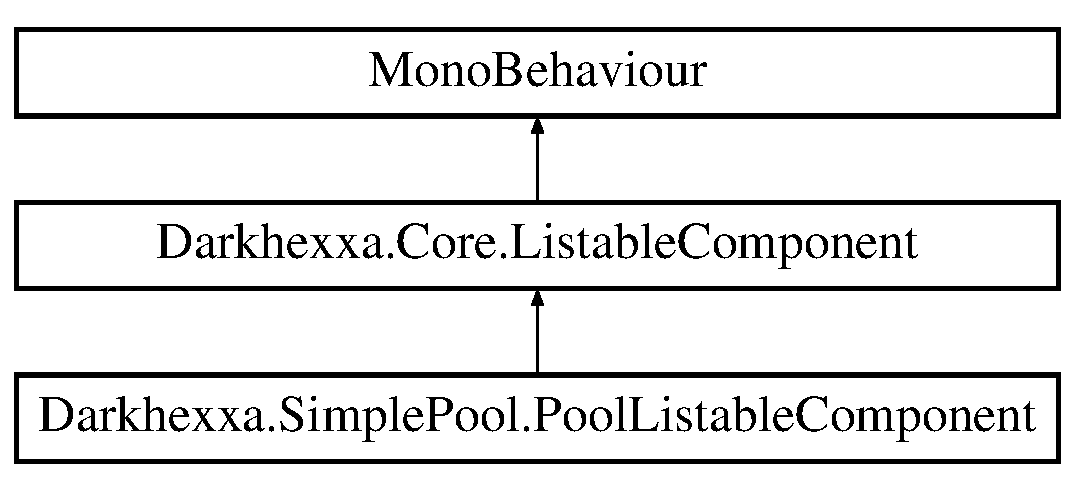
\includegraphics[height=3.000000cm]{class_darkhexxa_1_1_simple_pool_1_1_pool_listable_component}
\end{center}
\end{figure}
\subsection*{Additional Inherited Members}


\subsection{Detailed Description}
empty list class used to destinguash the pool lists from another list the objects might be in. 

Definition at line 21 of file Pool\-Listable\-Component.\-cs.



The documentation for this class was generated from the following file\-:\begin{DoxyCompactItemize}
\item 
C\-:/\-Users/\-Anthony/\-Game\-\_\-\-Development/\-Unity\-\_\-\-Projects/\-Darkhexxa/\-Assets/\-Darkhexxa/\-Simpel\-Pool/\-Components/\hyperlink{_pool_listable_component_8cs}{Pool\-Listable\-Component.\-cs}\end{DoxyCompactItemize}

\hypertarget{class_darkhexxa_1_1_simple_pool_1_1_simple_pool}{\section{Darkhexxa.\-Simple\-Pool.\-Simple\-Pool Class Reference}
\label{class_darkhexxa_1_1_simple_pool_1_1_simple_pool}\index{Darkhexxa.\-Simple\-Pool.\-Simple\-Pool@{Darkhexxa.\-Simple\-Pool.\-Simple\-Pool}}
}
Inheritance diagram for Darkhexxa.\-Simple\-Pool.\-Simple\-Pool\-:\begin{figure}[H]
\begin{center}
\leavevmode
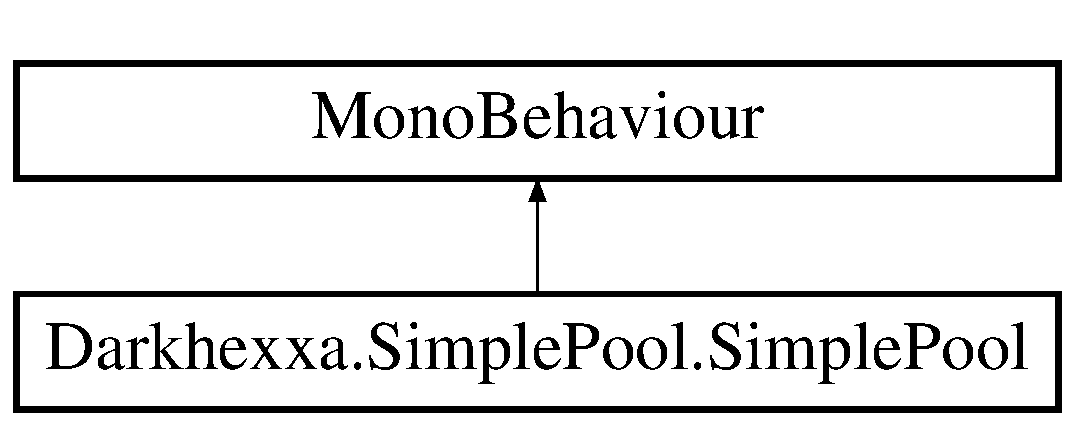
\includegraphics[height=2.000000cm]{class_darkhexxa_1_1_simple_pool_1_1_simple_pool}
\end{center}
\end{figure}
\subsection*{Classes}
\begin{DoxyCompactItemize}
\item 
class \hyperlink{class_darkhexxa_1_1_simple_pool_1_1_simple_pool_1_1_pool_data}{Pool\-Data}
\begin{DoxyCompactList}\small\item\em Data for the pool. \end{DoxyCompactList}\end{DoxyCompactItemize}
\subsection*{Public Member Functions}
\begin{DoxyCompactItemize}
\item 
Game\-Object \hyperlink{class_darkhexxa_1_1_simple_pool_1_1_simple_pool_a7f29a18dde77e02e1cdd8ebd69fb6659}{Spawn} ()
\begin{DoxyCompactList}\small\item\em spawns a prfab with the spawners position and rotation \end{DoxyCompactList}\item 
Game\-Object \hyperlink{class_darkhexxa_1_1_simple_pool_1_1_simple_pool_a30e8d7d6d02759f1d2de167a2c1d22e4}{Spawn} (Vector3 position, Quaternion rotation)
\begin{DoxyCompactList}\small\item\em spawns a clone at a given position and rotation \end{DoxyCompactList}\item 
void \hyperlink{class_darkhexxa_1_1_simple_pool_1_1_simple_pool_ace3fe63b086d4c556517b6f7070874d9}{Despawn} (Game\-Object obj)
\begin{DoxyCompactList}\small\item\em despawns on object \end{DoxyCompactList}\end{DoxyCompactItemize}
\subsection*{Static Public Member Functions}
\begin{DoxyCompactItemize}
\item 
static \hyperlink{class_darkhexxa_1_1_simple_pool_1_1_simple_pool}{Simple\-Pool} \hyperlink{class_darkhexxa_1_1_simple_pool_1_1_simple_pool_a160f842c9441fb80243a9813492e7d08}{Find\-Pool\-For} (Game\-Object prefab)
\begin{DoxyCompactList}\small\item\em static find function \end{DoxyCompactList}\item 
static \\*
System.\-Collections.\-Generic.\-I\-Enumerable\\*
$<$ \hyperlink{class_darkhexxa_1_1_simple_pool_1_1_simple_pool}{Simple\-Pool} $>$ \hyperlink{class_darkhexxa_1_1_simple_pool_1_1_simple_pool_a40a74364e51c2eedf108b8a375f22709}{Find\-All\-Pools\-For} (Game\-Object prefab)
\begin{DoxyCompactList}\small\item\em static find function \end{DoxyCompactList}\item 
static \hyperlink{class_darkhexxa_1_1_simple_pool_1_1_simple_pool}{Simple\-Pool} \hyperlink{class_darkhexxa_1_1_simple_pool_1_1_simple_pool_afbfdaaf049c575ddae1aa1343ddc08a5}{Find\-Pool\-For} (\hyperlink{class_darkhexxa_1_1_simple_pool_1_1_simple_pool_1_1_pool_data}{Pool\-Data} \hyperlink{class_darkhexxa_1_1_simple_pool_1_1_simple_pool_ae49843e11db3e9491d166dba366c3fdf}{data})
\begin{DoxyCompactList}\small\item\em static find function \end{DoxyCompactList}\item 
static \\*
System.\-Collections.\-Generic.\-I\-Enumerable\\*
$<$ \hyperlink{class_darkhexxa_1_1_simple_pool_1_1_simple_pool}{Simple\-Pool} $>$ \hyperlink{class_darkhexxa_1_1_simple_pool_1_1_simple_pool_ab29a9b60515daff5ac4ca620546e5fc9}{Find\-All\-Pools\-For} (\hyperlink{class_darkhexxa_1_1_simple_pool_1_1_simple_pool_1_1_pool_data}{Pool\-Data} \hyperlink{class_darkhexxa_1_1_simple_pool_1_1_simple_pool_ae49843e11db3e9491d166dba366c3fdf}{data})
\begin{DoxyCompactList}\small\item\em static find function \end{DoxyCompactList}\item 
static \hyperlink{class_darkhexxa_1_1_simple_pool_1_1_simple_pool}{Simple\-Pool} \hyperlink{class_darkhexxa_1_1_simple_pool_1_1_simple_pool_a857d7f94168bb44468149385efae0855}{Create\-Pool} (Game\-Object prefab)
\begin{DoxyCompactList}\small\item\em static create pool function \end{DoxyCompactList}\item 
static \hyperlink{class_darkhexxa_1_1_simple_pool_1_1_simple_pool}{Simple\-Pool} \hyperlink{class_darkhexxa_1_1_simple_pool_1_1_simple_pool_a03871bfb6c3c3e7c9a843a1b9f213bdc}{Create\-Pool} (Game\-Object prefab, int max\-Count, int batch\-Create\-Count, bool cull\-Inactive, float cull\-Interval)
\begin{DoxyCompactList}\small\item\em static create pool function \end{DoxyCompactList}\item 
static \hyperlink{class_darkhexxa_1_1_simple_pool_1_1_simple_pool}{Simple\-Pool} \hyperlink{class_darkhexxa_1_1_simple_pool_1_1_simple_pool_add1f33c5ffe05b3b02c723c4c3b73f0a}{Create\-Pool} (string game\-Object\-Name, Game\-Object prefab)
\begin{DoxyCompactList}\small\item\em static create pool function \end{DoxyCompactList}\item 
static \hyperlink{class_darkhexxa_1_1_simple_pool_1_1_simple_pool}{Simple\-Pool} \hyperlink{class_darkhexxa_1_1_simple_pool_1_1_simple_pool_aaca6d9386024a8b21caf25be6e12faee}{Create\-Pool} (string game\-Object\-Name, Game\-Object prefab, int max\-Count, int batch\-Create\-Count, bool cull\-Inactive, float cull\-Interval)
\begin{DoxyCompactList}\small\item\em static create pool function \end{DoxyCompactList}\item 
static \hyperlink{class_darkhexxa_1_1_simple_pool_1_1_simple_pool}{Simple\-Pool} \hyperlink{class_darkhexxa_1_1_simple_pool_1_1_simple_pool_acb1b2386d78e2c28b3432fc2fc46ee7e}{Create\-Pool} (\hyperlink{class_darkhexxa_1_1_simple_pool_1_1_simple_pool_1_1_pool_data}{Pool\-Data} \hyperlink{class_darkhexxa_1_1_simple_pool_1_1_simple_pool_ae49843e11db3e9491d166dba366c3fdf}{data})
\begin{DoxyCompactList}\small\item\em static create pool function \end{DoxyCompactList}\item 
static \hyperlink{class_darkhexxa_1_1_simple_pool_1_1_simple_pool}{Simple\-Pool} \hyperlink{class_darkhexxa_1_1_simple_pool_1_1_simple_pool_ac3275f8690158103e61659b48a3868da}{Create\-Pool} (string game\-Object\-Name, \hyperlink{class_darkhexxa_1_1_simple_pool_1_1_simple_pool_1_1_pool_data}{Pool\-Data} \hyperlink{class_darkhexxa_1_1_simple_pool_1_1_simple_pool_ae49843e11db3e9491d166dba366c3fdf}{data})
\begin{DoxyCompactList}\small\item\em static create pool function \end{DoxyCompactList}\end{DoxyCompactItemize}
\subsection*{Public Attributes}
\begin{DoxyCompactItemize}
\item 
\hyperlink{class_darkhexxa_1_1_simple_pool_1_1_simple_pool_1_1_pool_data}{Pool\-Data} \hyperlink{class_darkhexxa_1_1_simple_pool_1_1_simple_pool_ae49843e11db3e9491d166dba366c3fdf}{data} = new \hyperlink{class_darkhexxa_1_1_simple_pool_1_1_simple_pool_1_1_pool_data}{Pool\-Data}(null)
\begin{DoxyCompactList}\small\item\em Pool data object for this pool. \end{DoxyCompactList}\end{DoxyCompactItemize}


\subsection{Detailed Description}
Simple Pool Component give it a game object and it will spawn clones. 

Definition at line 17 of file Simple\-Pool.\-cs.



\subsection{Member Function Documentation}
\hypertarget{class_darkhexxa_1_1_simple_pool_1_1_simple_pool_a857d7f94168bb44468149385efae0855}{\index{Darkhexxa\-::\-Simple\-Pool\-::\-Simple\-Pool@{Darkhexxa\-::\-Simple\-Pool\-::\-Simple\-Pool}!Create\-Pool@{Create\-Pool}}
\index{Create\-Pool@{Create\-Pool}!Darkhexxa::SimplePool::SimplePool@{Darkhexxa\-::\-Simple\-Pool\-::\-Simple\-Pool}}
\subsubsection[{Create\-Pool}]{\setlength{\rightskip}{0pt plus 5cm}static {\bf Simple\-Pool} Darkhexxa.\-Simple\-Pool.\-Simple\-Pool.\-Create\-Pool (
\begin{DoxyParamCaption}
\item[{Game\-Object}]{prefab}
\end{DoxyParamCaption}
)\hspace{0.3cm}{\ttfamily [static]}}}\label{class_darkhexxa_1_1_simple_pool_1_1_simple_pool_a857d7f94168bb44468149385efae0855}


static create pool function 

searches for a similar pool if non is found it will create one. 
\begin{DoxyParams}{Parameters}
{\em Game\-Object} & the prefab of the pool you wish to find/create \\
\hline
\end{DoxyParams}
\begin{DoxyReturn}{Returns}
a matching pool or a new pool; 
\end{DoxyReturn}


Definition at line 396 of file Simple\-Pool.\-cs.

\hypertarget{class_darkhexxa_1_1_simple_pool_1_1_simple_pool_a03871bfb6c3c3e7c9a843a1b9f213bdc}{\index{Darkhexxa\-::\-Simple\-Pool\-::\-Simple\-Pool@{Darkhexxa\-::\-Simple\-Pool\-::\-Simple\-Pool}!Create\-Pool@{Create\-Pool}}
\index{Create\-Pool@{Create\-Pool}!Darkhexxa::SimplePool::SimplePool@{Darkhexxa\-::\-Simple\-Pool\-::\-Simple\-Pool}}
\subsubsection[{Create\-Pool}]{\setlength{\rightskip}{0pt plus 5cm}static {\bf Simple\-Pool} Darkhexxa.\-Simple\-Pool.\-Simple\-Pool.\-Create\-Pool (
\begin{DoxyParamCaption}
\item[{Game\-Object}]{prefab, }
\item[{int}]{max\-Count, }
\item[{int}]{batch\-Create\-Count, }
\item[{bool}]{cull\-Inactive, }
\item[{float}]{cull\-Interval}
\end{DoxyParamCaption}
)\hspace{0.3cm}{\ttfamily [static]}}}\label{class_darkhexxa_1_1_simple_pool_1_1_simple_pool_a03871bfb6c3c3e7c9a843a1b9f213bdc}


static create pool function 

searches for a similar pool if non is found it will create one. 
\begin{DoxyParams}{Parameters}
{\em Game\-Object} & the prefab of the pool you wish to find/create \\
\hline
{\em int} & maxium number of objects to clone \\
\hline
{\em int} & the number of objects to create when new objects are needed. \\
\hline
{\em bool} & cull the inactive objects on a set interval \\
\hline
{\em float} & the interval of the cull events. \\
\hline
\end{DoxyParams}
\begin{DoxyReturn}{Returns}
a matching pool or a new pool; 
\end{DoxyReturn}


Definition at line 413 of file Simple\-Pool.\-cs.

\hypertarget{class_darkhexxa_1_1_simple_pool_1_1_simple_pool_add1f33c5ffe05b3b02c723c4c3b73f0a}{\index{Darkhexxa\-::\-Simple\-Pool\-::\-Simple\-Pool@{Darkhexxa\-::\-Simple\-Pool\-::\-Simple\-Pool}!Create\-Pool@{Create\-Pool}}
\index{Create\-Pool@{Create\-Pool}!Darkhexxa::SimplePool::SimplePool@{Darkhexxa\-::\-Simple\-Pool\-::\-Simple\-Pool}}
\subsubsection[{Create\-Pool}]{\setlength{\rightskip}{0pt plus 5cm}static {\bf Simple\-Pool} Darkhexxa.\-Simple\-Pool.\-Simple\-Pool.\-Create\-Pool (
\begin{DoxyParamCaption}
\item[{string}]{game\-Object\-Name, }
\item[{Game\-Object}]{prefab}
\end{DoxyParamCaption}
)\hspace{0.3cm}{\ttfamily [static]}}}\label{class_darkhexxa_1_1_simple_pool_1_1_simple_pool_add1f33c5ffe05b3b02c723c4c3b73f0a}


static create pool function 

searches for a similar pool if non is found it will create one. 
\begin{DoxyParams}{Parameters}
{\em string} & name of the Game\-Object the pool component is attached to \\
\hline
{\em Game\-Object} & the prefab of the pool you wish to find/create \\
\hline
\end{DoxyParams}
\begin{DoxyReturn}{Returns}
a matching pool or a new pool; 
\end{DoxyReturn}


Definition at line 427 of file Simple\-Pool.\-cs.

\hypertarget{class_darkhexxa_1_1_simple_pool_1_1_simple_pool_aaca6d9386024a8b21caf25be6e12faee}{\index{Darkhexxa\-::\-Simple\-Pool\-::\-Simple\-Pool@{Darkhexxa\-::\-Simple\-Pool\-::\-Simple\-Pool}!Create\-Pool@{Create\-Pool}}
\index{Create\-Pool@{Create\-Pool}!Darkhexxa::SimplePool::SimplePool@{Darkhexxa\-::\-Simple\-Pool\-::\-Simple\-Pool}}
\subsubsection[{Create\-Pool}]{\setlength{\rightskip}{0pt plus 5cm}static {\bf Simple\-Pool} Darkhexxa.\-Simple\-Pool.\-Simple\-Pool.\-Create\-Pool (
\begin{DoxyParamCaption}
\item[{string}]{game\-Object\-Name, }
\item[{Game\-Object}]{prefab, }
\item[{int}]{max\-Count, }
\item[{int}]{batch\-Create\-Count, }
\item[{bool}]{cull\-Inactive, }
\item[{float}]{cull\-Interval}
\end{DoxyParamCaption}
)\hspace{0.3cm}{\ttfamily [static]}}}\label{class_darkhexxa_1_1_simple_pool_1_1_simple_pool_aaca6d9386024a8b21caf25be6e12faee}


static create pool function 

searches for a similar pool if non is found it will create one. 
\begin{DoxyParams}{Parameters}
{\em string} & name of the Game\-Object the pool component is attached to \\
\hline
{\em Game\-Object} & the prefab of the pool you wish to find/create \\
\hline
{\em int} & maxium number of objects to clone \\
\hline
{\em int} & the number of objects to create when new objects are needed. \\
\hline
{\em bool} & cull the inactive objects on a set interval \\
\hline
{\em float} & the interval of the cull events. \\
\hline
\end{DoxyParams}
\begin{DoxyReturn}{Returns}
a matching pool or a new pool; 
\end{DoxyReturn}


Definition at line 445 of file Simple\-Pool.\-cs.

\hypertarget{class_darkhexxa_1_1_simple_pool_1_1_simple_pool_acb1b2386d78e2c28b3432fc2fc46ee7e}{\index{Darkhexxa\-::\-Simple\-Pool\-::\-Simple\-Pool@{Darkhexxa\-::\-Simple\-Pool\-::\-Simple\-Pool}!Create\-Pool@{Create\-Pool}}
\index{Create\-Pool@{Create\-Pool}!Darkhexxa::SimplePool::SimplePool@{Darkhexxa\-::\-Simple\-Pool\-::\-Simple\-Pool}}
\subsubsection[{Create\-Pool}]{\setlength{\rightskip}{0pt plus 5cm}static {\bf Simple\-Pool} Darkhexxa.\-Simple\-Pool.\-Simple\-Pool.\-Create\-Pool (
\begin{DoxyParamCaption}
\item[{{\bf Pool\-Data}}]{data}
\end{DoxyParamCaption}
)\hspace{0.3cm}{\ttfamily [static]}}}\label{class_darkhexxa_1_1_simple_pool_1_1_simple_pool_acb1b2386d78e2c28b3432fc2fc46ee7e}


static create pool function 

searches for a similar pool if non is found it will create one. 
\begin{DoxyParams}{Parameters}
{\em \hyperlink{class_darkhexxa_1_1_simple_pool_1_1_simple_pool_1_1_pool_data}{Pool\-Data}} & object that is used to create the pool component. \\
\hline
\end{DoxyParams}
\begin{DoxyReturn}{Returns}
a matching pool or a new pool; 
\end{DoxyReturn}


Definition at line 458 of file Simple\-Pool.\-cs.

\hypertarget{class_darkhexxa_1_1_simple_pool_1_1_simple_pool_ac3275f8690158103e61659b48a3868da}{\index{Darkhexxa\-::\-Simple\-Pool\-::\-Simple\-Pool@{Darkhexxa\-::\-Simple\-Pool\-::\-Simple\-Pool}!Create\-Pool@{Create\-Pool}}
\index{Create\-Pool@{Create\-Pool}!Darkhexxa::SimplePool::SimplePool@{Darkhexxa\-::\-Simple\-Pool\-::\-Simple\-Pool}}
\subsubsection[{Create\-Pool}]{\setlength{\rightskip}{0pt plus 5cm}static {\bf Simple\-Pool} Darkhexxa.\-Simple\-Pool.\-Simple\-Pool.\-Create\-Pool (
\begin{DoxyParamCaption}
\item[{string}]{game\-Object\-Name, }
\item[{{\bf Pool\-Data}}]{data}
\end{DoxyParamCaption}
)\hspace{0.3cm}{\ttfamily [static]}}}\label{class_darkhexxa_1_1_simple_pool_1_1_simple_pool_ac3275f8690158103e61659b48a3868da}


static create pool function 

searches for a similar pool if non is found it will create one. 
\begin{DoxyParams}{Parameters}
{\em string} & name of the Game\-Object the pool component is attached to \\
\hline
{\em \hyperlink{class_darkhexxa_1_1_simple_pool_1_1_simple_pool_1_1_pool_data}{Pool\-Data}} & object that is used to create the pool component. \\
\hline
\end{DoxyParams}
\begin{DoxyReturn}{Returns}
a matching pool or a new pool; 
\end{DoxyReturn}


Definition at line 474 of file Simple\-Pool.\-cs.

\hypertarget{class_darkhexxa_1_1_simple_pool_1_1_simple_pool_ace3fe63b086d4c556517b6f7070874d9}{\index{Darkhexxa\-::\-Simple\-Pool\-::\-Simple\-Pool@{Darkhexxa\-::\-Simple\-Pool\-::\-Simple\-Pool}!Despawn@{Despawn}}
\index{Despawn@{Despawn}!Darkhexxa::SimplePool::SimplePool@{Darkhexxa\-::\-Simple\-Pool\-::\-Simple\-Pool}}
\subsubsection[{Despawn}]{\setlength{\rightskip}{0pt plus 5cm}void Darkhexxa.\-Simple\-Pool.\-Simple\-Pool.\-Despawn (
\begin{DoxyParamCaption}
\item[{Game\-Object}]{obj}
\end{DoxyParamCaption}
)}}\label{class_darkhexxa_1_1_simple_pool_1_1_simple_pool_ace3fe63b086d4c556517b6f7070874d9}


despawns on object 


\begin{DoxyParams}{Parameters}
{\em Game\-Object} & game objects to remove from the active scene. \\
\hline
\end{DoxyParams}


Definition at line 258 of file Simple\-Pool.\-cs.

\hypertarget{class_darkhexxa_1_1_simple_pool_1_1_simple_pool_a40a74364e51c2eedf108b8a375f22709}{\index{Darkhexxa\-::\-Simple\-Pool\-::\-Simple\-Pool@{Darkhexxa\-::\-Simple\-Pool\-::\-Simple\-Pool}!Find\-All\-Pools\-For@{Find\-All\-Pools\-For}}
\index{Find\-All\-Pools\-For@{Find\-All\-Pools\-For}!Darkhexxa::SimplePool::SimplePool@{Darkhexxa\-::\-Simple\-Pool\-::\-Simple\-Pool}}
\subsubsection[{Find\-All\-Pools\-For}]{\setlength{\rightskip}{0pt plus 5cm}static System.\-Collections.\-Generic.\-I\-Enumerable$<${\bf Simple\-Pool}$>$ Darkhexxa.\-Simple\-Pool.\-Simple\-Pool.\-Find\-All\-Pools\-For (
\begin{DoxyParamCaption}
\item[{Game\-Object}]{prefab}
\end{DoxyParamCaption}
)\hspace{0.3cm}{\ttfamily [static]}}}\label{class_darkhexxa_1_1_simple_pool_1_1_simple_pool_a40a74364e51c2eedf108b8a375f22709}


static find function 

Seaches though all pools in the scene for one that generates the prefab. 
\begin{DoxyParams}{Parameters}
{\em Game\-Object} & the prefab of the pool you wish to find \\
\hline
\end{DoxyParams}
\begin{DoxyReturn}{Returns}
I\-Enumerable$<$\-Simple\-Pool$>$ yielding all matching pools; 
\end{DoxyReturn}


Definition at line 335 of file Simple\-Pool.\-cs.

\hypertarget{class_darkhexxa_1_1_simple_pool_1_1_simple_pool_ab29a9b60515daff5ac4ca620546e5fc9}{\index{Darkhexxa\-::\-Simple\-Pool\-::\-Simple\-Pool@{Darkhexxa\-::\-Simple\-Pool\-::\-Simple\-Pool}!Find\-All\-Pools\-For@{Find\-All\-Pools\-For}}
\index{Find\-All\-Pools\-For@{Find\-All\-Pools\-For}!Darkhexxa::SimplePool::SimplePool@{Darkhexxa\-::\-Simple\-Pool\-::\-Simple\-Pool}}
\subsubsection[{Find\-All\-Pools\-For}]{\setlength{\rightskip}{0pt plus 5cm}static System.\-Collections.\-Generic.\-I\-Enumerable$<${\bf Simple\-Pool}$>$ Darkhexxa.\-Simple\-Pool.\-Simple\-Pool.\-Find\-All\-Pools\-For (
\begin{DoxyParamCaption}
\item[{{\bf Pool\-Data}}]{data}
\end{DoxyParamCaption}
)\hspace{0.3cm}{\ttfamily [static]}}}\label{class_darkhexxa_1_1_simple_pool_1_1_simple_pool_ab29a9b60515daff5ac4ca620546e5fc9}


static find function 

Seaches though all pools in the scene for one that has a similar \hyperlink{class_darkhexxa_1_1_simple_pool_1_1_simple_pool_1_1_pool_data}{Pool\-Data} block 
\begin{DoxyParams}{Parameters}
{\em Game\-Object} & the prefab of the pool you wish to find \\
\hline
\end{DoxyParams}
\begin{DoxyReturn}{Returns}
I\-Enumerable$<$\-Simple\-Pool$>$ yielding all matching pools; 
\end{DoxyReturn}


Definition at line 375 of file Simple\-Pool.\-cs.

\hypertarget{class_darkhexxa_1_1_simple_pool_1_1_simple_pool_a160f842c9441fb80243a9813492e7d08}{\index{Darkhexxa\-::\-Simple\-Pool\-::\-Simple\-Pool@{Darkhexxa\-::\-Simple\-Pool\-::\-Simple\-Pool}!Find\-Pool\-For@{Find\-Pool\-For}}
\index{Find\-Pool\-For@{Find\-Pool\-For}!Darkhexxa::SimplePool::SimplePool@{Darkhexxa\-::\-Simple\-Pool\-::\-Simple\-Pool}}
\subsubsection[{Find\-Pool\-For}]{\setlength{\rightskip}{0pt plus 5cm}static {\bf Simple\-Pool} Darkhexxa.\-Simple\-Pool.\-Simple\-Pool.\-Find\-Pool\-For (
\begin{DoxyParamCaption}
\item[{Game\-Object}]{prefab}
\end{DoxyParamCaption}
)\hspace{0.3cm}{\ttfamily [static]}}}\label{class_darkhexxa_1_1_simple_pool_1_1_simple_pool_a160f842c9441fb80243a9813492e7d08}


static find function 

Seaches though all pools in the scene for one that generates the prefab. 
\begin{DoxyParams}{Parameters}
{\em Game\-Object} & the prefab of the pool you wish to find \\
\hline
\end{DoxyParams}
\begin{DoxyReturn}{Returns}
a matching pool or null; 
\end{DoxyReturn}


Definition at line 315 of file Simple\-Pool.\-cs.

\hypertarget{class_darkhexxa_1_1_simple_pool_1_1_simple_pool_afbfdaaf049c575ddae1aa1343ddc08a5}{\index{Darkhexxa\-::\-Simple\-Pool\-::\-Simple\-Pool@{Darkhexxa\-::\-Simple\-Pool\-::\-Simple\-Pool}!Find\-Pool\-For@{Find\-Pool\-For}}
\index{Find\-Pool\-For@{Find\-Pool\-For}!Darkhexxa::SimplePool::SimplePool@{Darkhexxa\-::\-Simple\-Pool\-::\-Simple\-Pool}}
\subsubsection[{Find\-Pool\-For}]{\setlength{\rightskip}{0pt plus 5cm}static {\bf Simple\-Pool} Darkhexxa.\-Simple\-Pool.\-Simple\-Pool.\-Find\-Pool\-For (
\begin{DoxyParamCaption}
\item[{{\bf Pool\-Data}}]{data}
\end{DoxyParamCaption}
)\hspace{0.3cm}{\ttfamily [static]}}}\label{class_darkhexxa_1_1_simple_pool_1_1_simple_pool_afbfdaaf049c575ddae1aa1343ddc08a5}


static find function 

Seaches though all pools in the scene for one that has a similar \hyperlink{class_darkhexxa_1_1_simple_pool_1_1_simple_pool_1_1_pool_data}{Pool\-Data} block 
\begin{DoxyParams}{Parameters}
{\em Game\-Object} & the prefab of the pool you wish to find \\
\hline
\end{DoxyParams}
\begin{DoxyReturn}{Returns}
a matching pool or null; 
\end{DoxyReturn}


Definition at line 355 of file Simple\-Pool.\-cs.

\hypertarget{class_darkhexxa_1_1_simple_pool_1_1_simple_pool_a7f29a18dde77e02e1cdd8ebd69fb6659}{\index{Darkhexxa\-::\-Simple\-Pool\-::\-Simple\-Pool@{Darkhexxa\-::\-Simple\-Pool\-::\-Simple\-Pool}!Spawn@{Spawn}}
\index{Spawn@{Spawn}!Darkhexxa::SimplePool::SimplePool@{Darkhexxa\-::\-Simple\-Pool\-::\-Simple\-Pool}}
\subsubsection[{Spawn}]{\setlength{\rightskip}{0pt plus 5cm}Game\-Object Darkhexxa.\-Simple\-Pool.\-Simple\-Pool.\-Spawn (
\begin{DoxyParamCaption}
{}
\end{DoxyParamCaption}
)}}\label{class_darkhexxa_1_1_simple_pool_1_1_simple_pool_a7f29a18dde77e02e1cdd8ebd69fb6659}


spawns a prfab with the spawners position and rotation 



Definition at line 191 of file Simple\-Pool.\-cs.

\hypertarget{class_darkhexxa_1_1_simple_pool_1_1_simple_pool_a30e8d7d6d02759f1d2de167a2c1d22e4}{\index{Darkhexxa\-::\-Simple\-Pool\-::\-Simple\-Pool@{Darkhexxa\-::\-Simple\-Pool\-::\-Simple\-Pool}!Spawn@{Spawn}}
\index{Spawn@{Spawn}!Darkhexxa::SimplePool::SimplePool@{Darkhexxa\-::\-Simple\-Pool\-::\-Simple\-Pool}}
\subsubsection[{Spawn}]{\setlength{\rightskip}{0pt plus 5cm}Game\-Object Darkhexxa.\-Simple\-Pool.\-Simple\-Pool.\-Spawn (
\begin{DoxyParamCaption}
\item[{Vector3}]{position, }
\item[{Quaternion}]{rotation}
\end{DoxyParamCaption}
)}}\label{class_darkhexxa_1_1_simple_pool_1_1_simple_pool_a30e8d7d6d02759f1d2de167a2c1d22e4}


spawns a clone at a given position and rotation 


\begin{DoxyParams}{Parameters}
{\em position} & Vector3 position to spawn at \\
\hline
{\em rotation} & Quaternion rotation to set the new object to. \\
\hline
\end{DoxyParams}
\begin{DoxyReturn}{Returns}
Spawned Game Object; 
\end{DoxyReturn}


Definition at line 202 of file Simple\-Pool.\-cs.



\subsection{Member Data Documentation}
\hypertarget{class_darkhexxa_1_1_simple_pool_1_1_simple_pool_ae49843e11db3e9491d166dba366c3fdf}{\index{Darkhexxa\-::\-Simple\-Pool\-::\-Simple\-Pool@{Darkhexxa\-::\-Simple\-Pool\-::\-Simple\-Pool}!data@{data}}
\index{data@{data}!Darkhexxa::SimplePool::SimplePool@{Darkhexxa\-::\-Simple\-Pool\-::\-Simple\-Pool}}
\subsubsection[{data}]{\setlength{\rightskip}{0pt plus 5cm}{\bf Pool\-Data} Darkhexxa.\-Simple\-Pool.\-Simple\-Pool.\-data = new {\bf Pool\-Data}(null)}}\label{class_darkhexxa_1_1_simple_pool_1_1_simple_pool_ae49843e11db3e9491d166dba366c3fdf}


Pool data object for this pool. 



Definition at line 113 of file Simple\-Pool.\-cs.



The documentation for this class was generated from the following file\-:\begin{DoxyCompactItemize}
\item 
C\-:/\-Users/\-Anthony/\-Game\-\_\-\-Development/\-Unity\-\_\-\-Projects/\-Darkhexxa/\-Assets/\-Darkhexxa/\-Simpel\-Pool/\hyperlink{_simple_pool_8cs}{Simple\-Pool.\-cs}\end{DoxyCompactItemize}

\chapter{File Documentation}
\hypertarget{_array_helper_8cs}{\section{C\-:/\-Users/\-Anthony/\-Game\-\_\-\-Development/\-Unity\-\_\-\-Projects/\-Hostile/\-Assets/\-Hostile/\-Core/\-Array\-Helper.cs File Reference}
\label{_array_helper_8cs}\index{C\-:/\-Users/\-Anthony/\-Game\-\_\-\-Development/\-Unity\-\_\-\-Projects/\-Hostile/\-Assets/\-Hostile/\-Core/\-Array\-Helper.\-cs@{C\-:/\-Users/\-Anthony/\-Game\-\_\-\-Development/\-Unity\-\_\-\-Projects/\-Hostile/\-Assets/\-Hostile/\-Core/\-Array\-Helper.\-cs}}
}
\subsection*{Classes}
\begin{DoxyCompactItemize}
\item 
class {\bfseries Hostile.\-Core.\-Array\-Helper}
\end{DoxyCompactItemize}
\subsection*{Namespaces}
\begin{DoxyCompactItemize}
\item 
package \hyperlink{namespace_hostile}{Hostile}
\item 
package \hyperlink{namespace_hostile_1_1_core}{Hostile.\-Core}
\end{DoxyCompactItemize}

\hypertarget{_component_list_8cs}{\section{C\-:/\-Users/\-Anthony/\-Game\-\_\-\-Development/\-Unity\-\_\-\-Projects/\-Hostile/\-Assets/\-Hostile/\-Core/\-Component\-List.cs File Reference}
\label{_component_list_8cs}\index{C\-:/\-Users/\-Anthony/\-Game\-\_\-\-Development/\-Unity\-\_\-\-Projects/\-Hostile/\-Assets/\-Hostile/\-Core/\-Component\-List.\-cs@{C\-:/\-Users/\-Anthony/\-Game\-\_\-\-Development/\-Unity\-\_\-\-Projects/\-Hostile/\-Assets/\-Hostile/\-Core/\-Component\-List.\-cs}}
}
\subsection*{Classes}
\begin{DoxyCompactItemize}
\item 
class \hyperlink{class_hostile_1_1_core_1_1_component_list}{Hostile.\-Core.\-Component\-List}
\end{DoxyCompactItemize}
\subsection*{Namespaces}
\begin{DoxyCompactItemize}
\item 
package \hyperlink{namespace_hostile}{Hostile}
\item 
package \hyperlink{namespace_hostile_1_1_core}{Hostile.\-Core}
\end{DoxyCompactItemize}

\hypertarget{_listable_component_8cs}{\section{C\-:/\-Users/\-Anthony/\-Game\-\_\-\-Development/\-Unity\-\_\-\-Projects/\-Darkhexxa/\-Assets/\-Darkhexxa/\-Core/\-Listable\-Component.cs File Reference}
\label{_listable_component_8cs}\index{C\-:/\-Users/\-Anthony/\-Game\-\_\-\-Development/\-Unity\-\_\-\-Projects/\-Darkhexxa/\-Assets/\-Darkhexxa/\-Core/\-Listable\-Component.\-cs@{C\-:/\-Users/\-Anthony/\-Game\-\_\-\-Development/\-Unity\-\_\-\-Projects/\-Darkhexxa/\-Assets/\-Darkhexxa/\-Core/\-Listable\-Component.\-cs}}
}
\subsection*{Classes}
\begin{DoxyCompactItemize}
\item 
class \hyperlink{class_darkhexxa_1_1_core_1_1_listable_component}{Darkhexxa.\-Core.\-Listable\-Component}
\end{DoxyCompactItemize}
\subsection*{Namespaces}
\begin{DoxyCompactItemize}
\item 
package \hyperlink{namespace_darkhexxa}{Darkhexxa}
\item 
package \hyperlink{namespace_darkhexxa_1_1_core}{Darkhexxa.\-Core}
\end{DoxyCompactItemize}

\hypertarget{_base_pool_component_8cs}{\section{C\-:/\-Users/\-Anthony/\-Game\-\_\-\-Development/\-Unity\-\_\-\-Projects/\-Darkhexxa/\-Assets/\-Darkhexxa/\-Simpel\-Pool/\-Components/\-Base\-Pool\-Component.cs File Reference}
\label{_base_pool_component_8cs}\index{C\-:/\-Users/\-Anthony/\-Game\-\_\-\-Development/\-Unity\-\_\-\-Projects/\-Darkhexxa/\-Assets/\-Darkhexxa/\-Simpel\-Pool/\-Components/\-Base\-Pool\-Component.\-cs@{C\-:/\-Users/\-Anthony/\-Game\-\_\-\-Development/\-Unity\-\_\-\-Projects/\-Darkhexxa/\-Assets/\-Darkhexxa/\-Simpel\-Pool/\-Components/\-Base\-Pool\-Component.\-cs}}
}
\subsection*{Classes}
\begin{DoxyCompactItemize}
\item 
class \hyperlink{class_darkhexxa_1_1_simple_pool_1_1_components_1_1_base_pool_component}{Darkhexxa.\-Simple\-Pool.\-Components.\-Base\-Pool\-Component}
\begin{DoxyCompactList}\small\item\em Abstact Base class for Game\-Objects created by pools. \end{DoxyCompactList}\end{DoxyCompactItemize}
\subsection*{Namespaces}
\begin{DoxyCompactItemize}
\item 
package \hyperlink{namespace_darkhexxa}{Darkhexxa}
\item 
package \hyperlink{namespace_darkhexxa_1_1_simple_pool}{Darkhexxa.\-Simple\-Pool}
\item 
package \hyperlink{namespace_darkhexxa_1_1_simple_pool_1_1_components}{Darkhexxa.\-Simple\-Pool.\-Components}
\end{DoxyCompactItemize}

\hypertarget{_cull_off_screen_8cs}{\section{C\-:/\-Users/\-Anthony/\-Game\-\_\-\-Development/\-Unity\-\_\-\-Projects/\-Hostile/\-Assets/\-Hostile/\-Simpel\-Pool/\-Components/\-Cull\-Off\-Screen.cs File Reference}
\label{_cull_off_screen_8cs}\index{C\-:/\-Users/\-Anthony/\-Game\-\_\-\-Development/\-Unity\-\_\-\-Projects/\-Hostile/\-Assets/\-Hostile/\-Simpel\-Pool/\-Components/\-Cull\-Off\-Screen.\-cs@{C\-:/\-Users/\-Anthony/\-Game\-\_\-\-Development/\-Unity\-\_\-\-Projects/\-Hostile/\-Assets/\-Hostile/\-Simpel\-Pool/\-Components/\-Cull\-Off\-Screen.\-cs}}
}
\subsection*{Classes}
\begin{DoxyCompactItemize}
\item 
class \hyperlink{class_hostile_1_1_simple_pool_1_1_components_1_1_cull_off_screen}{Hostile.\-Simple\-Pool.\-Components.\-Cull\-Off\-Screen}
\begin{DoxyCompactList}\small\item\em A base pool component that despawns the attached object when it goes off screen. \end{DoxyCompactList}\end{DoxyCompactItemize}
\subsection*{Namespaces}
\begin{DoxyCompactItemize}
\item 
package \hyperlink{namespace_hostile}{Hostile}
\item 
package \hyperlink{namespace_hostile_1_1_simple_pool}{Hostile.\-Simple\-Pool}
\item 
package \hyperlink{namespace_hostile_1_1_simple_pool_1_1_components}{Hostile.\-Simple\-Pool.\-Components}
\end{DoxyCompactItemize}

\hypertarget{_pool_listable_component_8cs}{\section{C\-:/\-Users/\-Anthony/\-Game\-\_\-\-Development/\-Unity\-\_\-\-Projects/\-Darkhexxa/\-Assets/\-Darkhexxa/\-Simpel\-Pool/\-Components/\-Pool\-Listable\-Component.cs File Reference}
\label{_pool_listable_component_8cs}\index{C\-:/\-Users/\-Anthony/\-Game\-\_\-\-Development/\-Unity\-\_\-\-Projects/\-Darkhexxa/\-Assets/\-Darkhexxa/\-Simpel\-Pool/\-Components/\-Pool\-Listable\-Component.\-cs@{C\-:/\-Users/\-Anthony/\-Game\-\_\-\-Development/\-Unity\-\_\-\-Projects/\-Darkhexxa/\-Assets/\-Darkhexxa/\-Simpel\-Pool/\-Components/\-Pool\-Listable\-Component.\-cs}}
}
\subsection*{Classes}
\begin{DoxyCompactItemize}
\item 
class \hyperlink{class_darkhexxa_1_1_simple_pool_1_1_pool_listable_component}{Darkhexxa.\-Simple\-Pool.\-Pool\-Listable\-Component}
\begin{DoxyCompactList}\small\item\em empty list class used to destinguash the pool lists from another list the objects might be in. \end{DoxyCompactList}\end{DoxyCompactItemize}
\subsection*{Namespaces}
\begin{DoxyCompactItemize}
\item 
package \hyperlink{namespace_darkhexxa}{Darkhexxa}
\item 
package \hyperlink{namespace_darkhexxa_1_1_simple_pool}{Darkhexxa.\-Simple\-Pool}
\end{DoxyCompactItemize}

\hypertarget{_simple_pool_8cs}{\section{C\-:/\-Users/\-Anthony/\-Game\-\_\-\-Development/\-Unity\-\_\-\-Projects/\-Darkhexxa/\-Assets/\-Darkhexxa/\-Simpel\-Pool/\-Simple\-Pool.cs File Reference}
\label{_simple_pool_8cs}\index{C\-:/\-Users/\-Anthony/\-Game\-\_\-\-Development/\-Unity\-\_\-\-Projects/\-Darkhexxa/\-Assets/\-Darkhexxa/\-Simpel\-Pool/\-Simple\-Pool.\-cs@{C\-:/\-Users/\-Anthony/\-Game\-\_\-\-Development/\-Unity\-\_\-\-Projects/\-Darkhexxa/\-Assets/\-Darkhexxa/\-Simpel\-Pool/\-Simple\-Pool.\-cs}}
}
\subsection*{Classes}
\begin{DoxyCompactItemize}
\item 
class \hyperlink{class_darkhexxa_1_1_simple_pool_1_1_simple_pool}{Darkhexxa.\-Simple\-Pool.\-Simple\-Pool}
\item 
class \hyperlink{class_darkhexxa_1_1_simple_pool_1_1_simple_pool_1_1_pool_data}{Darkhexxa.\-Simple\-Pool.\-Simple\-Pool.\-Pool\-Data}
\begin{DoxyCompactList}\small\item\em Data for the pool. \end{DoxyCompactList}\end{DoxyCompactItemize}
\subsection*{Namespaces}
\begin{DoxyCompactItemize}
\item 
package \hyperlink{namespace_darkhexxa}{Darkhexxa}
\item 
package \hyperlink{namespace_darkhexxa_1_1_simple_pool}{Darkhexxa.\-Simple\-Pool}
\end{DoxyCompactItemize}

%--- End generated contents ---

% Index
\newpage
\phantomsection
\addcontentsline{toc}{chapter}{Index}
\printindex

\end{document}
